\documentclass[12pt,oneside,a4paper]{article}
\usepackage{./custom}
\usepackage{listings}
\usepackage{color}
\usepackage{minted}
\usepackage{fvextra}
\usepackage{mdframed}
\usemintedstyle{pastie}
\usepackage[light, frenchstyle,narrowiints,partialup,notextcomp]{kpfonts}



\begin{document}
% title (fold)
\begin{titlepage}
\begin{center}

% Upper part of the page. The '~' is needed because \\
% only works if a paragraph has started.

\includegraphics[scale=0.4]{./img/logo_centralesup.jpg} \\[1.5cm]

% \textsc{\LARGE \textsc{CentraleSupélec}}\\[1.5cm]


\vfill
% Title
\rule{\textwidth}{1.6pt}\vspace*{-\baselineskip}\vspace*{2pt} % Thick horizontal line
\rule{\textwidth}{0.4pt}\\[\baselineskip] % Thin horizontal line
{ \huge \bfseries Travaux Pratiques \\ Modélisation de Risques Financiers \\[0.4cm] }
\rule{\textwidth}{0.4pt}\vspace*{-\baselineskip}\vspace{3.2pt} % Thin horizontal line
\rule{\textwidth}{1.6pt}\\[1.5cm] % Thick horizontal line

\vfill

\includegraphics[scale=0.8]{./img/bolsa} \\[1.5cm]

\vfill
% Author
{\large
\begin{center}
  % \adfast{1}  \hspace{0.5cm}\textsc{\textbf{Encadrant du projet}}\hspace{0.5cm}   \adfast{1}  \\[0.3cm] \large
  {\Large  \hspace{0.5cm} \textbf{Auteurs} \hspace{0.5cm}   } \\[0.3cm]
  % \adfast{1}  \hspace{0.5cm}\textsc{Nom des élèves} \hspace{0.5cm}   \adfast{1} \\[0.3cm] \large
	\textsc{Bataillou Almagro} Marc --- \textsc{Cobas Aranguren} Luís\\
	  ---
\end{center}
}
\vfill

% Bottom of the page
{\large 2016}

\end{center}
\end{titlepage}
% title (end) 

{\hypersetup{linkcolor=black}
\tableofcontents}
\newpage
{\hypersetup{linkcolor=black}
\listoffigures}
\newpage
\renewcommand\listoflistingscaption{Codes}
{\hypersetup{linkcolor=black}\listoflistings}
\newpage

\section{Formule de Black et Scholes} % (fold)
\label{sec:question_1}

Les fonctions permettant de calculer les différents influences et valeurs de cette section sont Listing~\ref{listing:10}.

Nous présentons dans les Figure~\ref{fig:call_s}, Figure~\ref{fig:call_sigma}, et Figure~\ref{fig:call_t}, l'évolution du prix d'un $CALL$ évalué selon la formule de Black et Scholes.

\begin{equation} C_{t}=S_{t}N(d_{1})-Ke^{-r(T-t)}N(d_{2})\end{equation}
où

\begin{align*}
N(d) &= \frac{1}{\sqrt{2\pi}}\int_{-\infty}^{d} {e^{\frac{-q^{2}}{2}} dq}\\\ 
d_1 &=\frac{1}{\sigma\sqrt{T-t}}(ln(\frac{S}{K})+(r+\frac{\sigma^{2}}{2})(T-t))\\
d_2 &=d_1-\sigma\sqrt{T-t}
\end{align*}

 On pourra se référer au document \textsc{black$\_$scholes.m} pour analyser l'implémentation de la formule sous \textsc{Matlab}. Pour simuler ce prix, on va prendre les paramètres suivants: le prix du sous-jacent $S_0=75$, le Strike $K=75$, l'échéance $T=1$, la volatilité $\sigma = 0.17$ et le taux d-actialisation $r=0.01$.
Avec ces paramètres, on obtient le prix d'un call européen $P_{B-S}=5.437$ en applicant le formule de Black et Scholes. 

\vfill

\begin{figure}[H]
\centering
% This file was created by matlab2tikz.
%
%The latest updates can be retrieved from
%  http://www.mathworks.com/matlabcentral/fileexchange/22022-matlab2tikz-matlab2tikz
%where you can also make suggestions and rate matlab2tikz.
%
\begin{tikzpicture}

\begin{axis}[%
width=0.6\linewidth,
height=0.6\linewidth,
at={(1.011in,0.642in)},
scale only axis,
xmin=0,
xmax=150,
xlabel style={font=\color{white!15!black}},
xlabel={$\text{S}_\text{0}$},
ymin=0,
ymax=80,
ylabel style={font=\color{white!15!black}},
ylabel={CALL},
axis background/.style={fill=white}
]
\addplot [color=black, line width=0.8pt, forget plot]
  table[row sep=crcr]{%
1	3.48452696036907e-143\\
1.5	5.32600750164986e-118\\
2	1.26513108472006e-101\\
2.5	8.94026972934864e-90\\
3	1.20260833302136e-80\\
3.5	2.57512625343218e-73\\
4	2.97861317801596e-67\\
4.5	3.99205620062664e-62\\
5	1.02853963445346e-57\\
5.5	7.24220129373355e-54\\
6	1.79588886128879e-50\\
6.5	1.89340652279537e-47\\
7	9.79573527802002e-45\\
7.5	2.78015911958792e-42\\
8	4.7277447299704e-40\\
8.5	5.17109753032313e-38\\
9	3.85425995649898e-36\\
9.5	2.05309577204604e-34\\
10	8.13237705632921e-33\\
10.5	2.4766110303593e-31\\
11	5.96517254319488e-30\\
11.5	1.16418294485456e-28\\
12	1.87974057884603e-27\\
12.5	2.5567560764831e-26\\
13	2.9759379630785e-25\\
13.5	3.00527432039802e-24\\
14	2.665246655631e-23\\
14.5	2.09818058683012e-22\\
15	1.48026429914428e-21\\
15.5	9.43882198771932e-21\\
16	5.48128912012728e-20\\
16.5	2.91878555260458e-19\\
17	1.43400681807623e-18\\
17.5	6.53654033555242e-18\\
18	2.7783353102926e-17\\
18.5	1.1062525330171e-16\\
19	4.14355545212528e-16\\
19.5	1.46555034040817e-15\\
20	4.91198049836248e-15\\
20.5	1.56507593585234e-14\\
21	4.75466130711325e-14\\
21.5	1.38099123228189e-13\\
22	3.8445049322425e-13\\
22.5	1.02819882878888e-12\\
23	2.64749873185482e-12\\
23.5	6.57633366594322e-12\\
24	1.57880162878873e-11\\
24.5	3.66958864119078e-11\\
25	8.27090103750631e-11\\
25.5	1.8104513906841e-10\\
26	3.85416095545765e-10\\
26.5	7.99011370906182e-10\\
27	1.61507033292347e-09\\
27.5	3.18674573336951e-09\\
28	6.14458397481216e-09\\
28.5	1.15896434868453e-08\\
29	2.14041291435038e-08\\
29.5	3.87407650857148e-08\\
30	6.8778525522472e-08\\
30.5	1.1986757138566e-07\\
31	2.05232239122842e-07\\
31.5	3.45459710618581e-07\\
32	5.72075528731744e-07\\
32.5	9.32597178113048e-07\\
33	1.49756490395498e-06\\
33.5	2.37017557071811e-06\\
34	3.69929062465313e-06\\
34.5	5.6967520313188e-06\\
35	8.66011808261261e-06\\
35.5	1.30021204741038e-05\\
36	1.92883398043171e-05\\
36.5	2.82847918731098e-05\\
37	4.10173036194069e-05\\
37.5	5.88447256981322e-05\\
38	8.35481679745541e-05\\
38.5	0.000117438543361212\\
39	0.000163484752970889\\
39.5	0.000225464830347128\\
40	0.00030814227427732\\
40.5	0.000417469629572665\\
41	0.000560821116434046\\
41.5	0.000747255757396752\\
42	0.000987812005157143\\
42.5	0.0012958343369803\\
43	0.0016873316575745\\
43.5	0.00218136665162482\\
44	0.00280047446244665\\
44.5	0.00357110826055682\\
45	0.00452410842431851\\
45.5	0.00569519120545953\\
46	0.00712545191808037\\
46.5	0.00886187689457257\\
47	0.0109578577195239\\
47.5	0.0134737006063819\\
48	0.0164771232429652\\
48.5	0.0200437310202536\\
49	0.0242574642905188\\
49.5	0.0292110081887073\\
50	0.0350061566037896\\
50.5	0.0417541221091475\\
51	0.0495757840530513\\
51.5	0.0586018675675375\\
52	0.0689730469678089\\
52.5	0.0808399678721332\\
53	0.0943631833574936\\
53.5	0.109713000559963\\
54	0.127069235308519\\
54.5	0.146620873623371\\
55	0.168565640189554\\
55.5	0.193109475208207\\
56	0.220465922305986\\
56.5	0.25085543142332\\
57	0.284504581780979\\
57.5	0.321645231120943\\
58	0.362513598412619\\
58.5	0.407349288092898\\
59	0.45639426465533\\
59.5	0.509891787009454\\
60	0.568085312489308\\
60.5	0.631217380696946\\
61	0.699528487521156\\
61.5	0.773255959676996\\
62	0.852632839972159\\
62.5	0.937886793230243\\
63	1.02923904239796\\
63.5	1.12690334384461\\
64	1.23108501024167\\
64.5	1.34197998870087\\
65	1.45977400106727\\
65.5	1.58464175242322\\
66	1.7167462129764\\
66.5	1.85623797759459\\
67	2.00325470632665\\
67.5	2.15792064832686\\
68	2.32034625069177\\
68.5	2.49062785283604\\
69	2.668847466188\\
69.5	2.85507263818527\\
70	3.0493563988044\\
70.5	3.25173728717177\\
71	3.46223945518204\\
71.5	3.68087284449808\\
72	3.90763343282542\\
72.5	4.14250354494638\\
73	4.38545222366307\\
73.5	4.63643565553483\\
74	4.89539764610137\\
74.5	5.16227013915577\\
75	5.43697377456752\\
75.5	5.71941847915171\\
76	6.00950408513145\\
76.5	6.30712097084087\\
77	6.61215071846256\\
77.5	6.92446678377892\\
78	7.24393517313696\\
78.5	7.57041512307599\\
79	7.90375977834112\\
79.5	8.24381686429867\\
80	8.59042935007648\\
80.5	8.94343609906976\\
81	9.30267250377535\\
81.5	9.66797110224302\\
82	10.0391621737541\\
82.5	10.4160743116574\\
83	10.7985349716013\\
83.5	11.1863709937031\\
84	11.5794090974835\\
84.5	11.9774763486689\\
85	12.3804005972239\\
85.5	12.7880108862167\\
86	13.2001378313502\\
86.5	13.616613971192\\
87	14.0372740883327\\
87.5	14.4619555018702\\
88	14.8904983317697\\
88.5	15.322745735789\\
89	15.7585441197714\\
89.5	16.1977433222165\\
90	16.64019677412\\
90.5	17.0857616351474\\
91	17.534298907261\\
91.5	17.9856735269652\\
92	18.4397544373629\\
92.5	18.8964146412374\\
93	19.3555312363815\\
93.5	19.8169854343963\\
94	20.2806625641717\\
94.5	20.7464520612442\\
95	21.2142474442043\\
95.5	21.6839462792975\\
96	22.1554501343258\\
96.5	22.6286645229214\\
97	23.103498840221\\
97.5	23.5798662909231\\
98	24.0576838106659\\
98.5	24.5368719816149\\
99	25.0173549430976\\
99.5	25.4990602980747\\
100	25.9819190161881\\
100.5	26.465865334072\\
101	26.9508366535693\\
101.5	27.4367734384434\\
102	27.9236191101299\\
102.5	28.4113199430269\\
103	28.8998249597779\\
103.5	29.3890858269596\\
104	29.8790567515443\\
104.5	30.369694378471\\
105	30.8609576896191\\
105.5	31.3528079044457\\
106	31.845208382515\\
106.5	32.3381245281161\\
107	32.831523697138\\
107.5	33.3253751063431\\
108	33.8196497451569\\
108.5	34.3143202900668\\
109	34.809361021704\\
109.5	35.304747744662\\
110	35.8004577100867\\
110.5	36.2964695410608\\
111	36.7927631607856\\
111.5	37.2893197235561\\
112	37.7861215485076\\
112.5	38.283152056108\\
113	38.780395707357\\
113.5	39.2778379456456\\
114	39.775465141225\\
114.5	40.2732645382264\\
115	40.7712242041681\\
115.5	41.2693329818834\\
116	41.7675804437981\\
116.5	42.265956848486\\
117	42.764453099426\\
117.5	43.263060705885\\
118	43.7617717458504\\
118.5	44.2605788309325\\
119	44.7594750731615\\
119.5	45.2584540536004\\
120	45.7575097926983\\
120.5	46.2566367223079\\
121	46.7558296592937\\
121.5	47.2550837806576\\
122	47.7543946001111\\
122.5	48.2537579460249\\
123	48.7531699406881\\
123.5	49.2526269808119\\
124	49.7521257192145\\
124.5	50.2516630476256\\
125	50.7512360805527\\
125.5	51.2508421401503\\
126	51.7504787420398\\
126.5	52.2501435820265\\
127	52.7498345236632\\
127.5	53.2495495866132\\
128	53.7492869357672\\
128.5	54.2490448710688\\
129	54.748821818009\\
129.5	55.2486163187477\\
130	55.7484270238275\\
130.5	56.2482526844406\\
131	56.7480921452178\\
131.5	57.2479443375052\\
132	57.7478082731003\\
132.5	58.2476830384161\\
133	58.7475677890482\\
133.5	59.2474617447184\\
134	59.74736418457\\
134.5	60.2472744427925\\
135	60.7471919045547\\
135.5	61.2471160022241\\
136	61.7470462118557\\
136.5	62.2469820499312\\
137	62.7469230703309\\
137.5	63.246868861525\\
138	63.7468190439664\\
138.5	64.2467732676736\\
139	64.7467312099894\\
139.5	65.2466925735032\\
140	65.7466570841264\\
140.5	66.2466244893094\\
141	66.74659455639\\
141.5	67.2465670710652\\
142	67.7465418359759\\
142.5	68.2465186693983\\
143	68.7464974040324\\
143.5	69.2464778858825\\
144	69.7464599732216\\
144.5	70.2464435356346\\
145	70.7464284531333\\
145.5	71.2464146153402\\
146	71.7464019207329\\
146.5	72.2463902759479\\
147	72.7463795951368\\
147.5	73.2463697993724\\
148	73.7463608161009\\
148.5	74.246352578636\\
149	74.7463450256926\\
149.5	75.2463381009567\\
150	75.7463317526884\\
};
\end{axis}
\end{tikzpicture}%
\caption{Variation du prix du CALL en fonction du sous-jacent $S_0$}
\label{fig:call_s}
\end{figure}

On voit une fonction convexe croissante en fonction de l'evolution de $S_{0}$. On remarque par ailleurs que la courbe tend vers la droite  $(S_{0}-K)_+$.

\vfill

\newpage

\begin{figure}[H]
\centering
% This file was created by matlab2tikz.
%
%The latest updates can be retrieved from
%  http://www.mathworks.com/matlabcentral/fileexchange/22022-matlab2tikz-matlab2tikz
%where you can also make suggestions and rate matlab2tikz.
%
\begin{tikzpicture}

\begin{axis}[%
width=0.6\linewidth,
height=0.6\linewidth,
at={(1.011in,0.642in)},
scale only axis,
xmin=0,
xmax=0.5,
xlabel style={font=\color{white!15!black}},
xlabel={$\sigma$},
ymin=0,
ymax=16,
ylabel style={font=\color{white!15!black}},
ylabel={CALL},
axis background/.style={fill=white}
]
\addplot [color=black, line width=0.8pt, forget plot]
  table[row sep=crcr]{%
0	0.74626246881239\\
0.001	0.74626246881239\\
0.002	0.746262476791642\\
0.003	0.746287560538804\\
0.004	0.746860710267867\\
0.005	0.749430594175749\\
0.006	0.755139888839224\\
0.007	0.764243344272899\\
0.008	0.776463043016619\\
0.009	0.791345899730914\\
0.01	0.808436925198144\\
0.011	0.827339593365011\\
0.012	0.847727179555896\\
0.013	0.869336547244295\\
0.014	0.891957364414637\\
0.015	0.915421497923134\\
0.016	0.939594015053757\\
0.017	0.964365983369404\\
0.018	0.9896488543339\\
0.019	1.01537012668518\\
0.02	1.04147000569575\\
0.021	1.06789882455645\\
0.022	1.09461504534421\\
0.023	1.12158370049652\\
0.024	1.14877516997301\\
0.025	1.17616421538088\\
0.026	1.2037292118989\\
0.027	1.23145153339492\\
0.028	1.25931505695296\\
0.029	1.28730576108205\\
0.03	1.3154113978977\\
0.031	1.34362122408398\\
0.032	1.37192577885259\\
0.033	1.40031669970256\\
0.034	1.42878656875946\\
0.035	1.45732878398898\\
0.036	1.48593745075294\\
0.037	1.51460729008613\\
0.038	1.54333356078458\\
0.039	1.57211199295563\\
0.04	1.60093873112323\\
0.041	1.62981028533267\\
0.042	1.65872348898058\\
0.043	1.68767546232123\\
0.044	1.71666358078188\\
0.045	1.74568544736729\\
0.046	1.77473886855395\\
0.047	1.80382183317165\\
0.048	1.8329324938513\\
0.049	1.86206915068387\\
0.05	1.89123023679011\\
0.051	1.92041430554635\\
0.052	1.9496200192496\\
0.053	1.97884613903684\\
0.054	2.00809151590011\\
0.055	2.03735508266127\\
0.056	2.06663584678936\\
0.057	2.09593288395933\\
0.058	2.12524533226471\\
0.059	2.15457238700821\\
0.06	2.18391329600418\\
0.061	2.21326735533541\\
0.062	2.24263390551378\\
0.063	2.27201232800101\\
0.064	2.30140204205045\\
0.065	2.3308025018362\\
0.066	2.3602131938395\\
0.067	2.38963363446589\\
0.068	2.41906336786987\\
0.069	2.44850196396623\\
0.07	2.47794901660968\\
0.071	2.50740414192642\\
0.072	2.53686697678317\\
0.073	2.56633717738045\\
0.074	2.59581441795878\\
0.075	2.62529838960715\\
0.076	2.65478879916453\\
0.077	2.68428536820625\\
0.078	2.71378783210745\\
0.079	2.74329593917685\\
0.08	2.7728094498552\\
0.081	2.80232813597217\\
0.082	2.83185178005738\\
0.083	2.86138017470066\\
0.084	2.89091312195773\\
0.085	2.92045043279732\\
0.086	2.94999192658669\\
0.087	2.97953743061227\\
0.088	3.00908677963272\\
0.089	3.03863981546198\\
0.09	3.06819638657976\\
0.091	3.09775634776767\\
0.092	3.1273195597688\\
0.093	3.1568858889692\\
0.094	3.18645520709947\\
0.095	3.21602739095514\\
0.096	3.24560232213433\\
0.097	3.27517988679165\\
0.098	3.30475997540695\\
0.099	3.33434248256808\\
0.1	3.36392730676656\\
0.101	3.39351435020537\\
0.102	3.4231035186179\\
0.103	3.45269472109749\\
0.104	3.48228786993665\\
0.105	3.51188288047546\\
0.106	3.54147967095856\\
0.107	3.5710781624\\
0.108	3.60067827845565\\
0.109	3.63027994530259\\
0.11	3.659883091525\\
0.111	3.68948764800625\\
0.112	3.71909354782663\\
0.113	3.74870072616665\\
0.114	3.77830912021534\\
0.115	3.80791866908316\\
0.116	3.83752931371967\\
0.117	3.8671409968352\\
0.118	3.89675366282653\\
0.119	3.92636725770637\\
0.12	3.95598172903625\\
0.121	3.98559702586283\\
0.122	4.01521309865722\\
0.123	4.04482989925737\\
0.124	4.07444738081306\\
0.125	4.10406549773379\\
0.126	4.13368420563881\\
0.127	4.16330346130985\\
0.128	4.19292322264573\\
0.129	4.22254344861933\\
0.13	4.25216409923641\\
0.131	4.28178513549629\\
0.132	4.31140651935444\\
0.133	4.34102821368662\\
0.134	4.37065018225465\\
0.135	4.4002723896738\\
0.136	4.42989480138143\\
0.137	4.45951738360719\\
0.138	4.48914010334436\\
0.139	4.51876292832254\\
0.14	4.54838582698137\\
0.141	4.57800876844555\\
0.142	4.60763172250078\\
0.143	4.63725465957067\\
0.144	4.66687755069476\\
0.145	4.69650036750735\\
0.146	4.72612308221719\\
0.147	4.75574566758799\\
0.148	4.78536809691987\\
0.149	4.81499034403127\\
0.15	4.84461238324184\\
0.151	4.87423418935595\\
0.152	4.9038557376467\\
0.153	4.93347700384078\\
0.154	4.9630979641037\\
0.155	4.99271859502581\\
0.156	5.02233887360863\\
0.157	5.05195877725195\\
0.158	5.08157828374113\\
0.159	5.11119737123516\\
0.16	5.14081601825497\\
0.161	5.17043420367227\\
0.162	5.20005190669877\\
0.163	5.22966910687581\\
0.164	5.25928578406436\\
0.165	5.28890191843536\\
0.166	5.31851749046048\\
0.167	5.34813248090314\\
0.168	5.37774687080986\\
0.169	5.40736064150197\\
0.17	5.43697377456752\\
0.171	5.46658625185357\\
0.172	5.49619805545875\\
0.173	5.52580916772588\\
0.174	5.5554195712352\\
0.175	5.58502924879744\\
0.176	5.61463818344747\\
0.177	5.64424635843792\\
0.178	5.67385375723311\\
0.179	5.70346036350323\\
0.18	5.73306616111863\\
0.181	5.76267113414431\\
0.182	5.79227526683467\\
0.183	5.82187854362832\\
0.184	5.85148094914314\\
0.185	5.88108246817148\\
0.186	5.91068308567552\\
0.187	5.94028278678271\\
0.188	5.96988155678147\\
0.189	5.99947938111699\\
0.19	6.02907624538704\\
0.191	6.05867213533816\\
0.192	6.08826703686167\\
0.193	6.11786093599009\\
0.194	6.14745381889343\\
0.195	6.1770456718758\\
0.196	6.20663648137197\\
0.197	6.23622623394407\\
0.198	6.26581491627847\\
0.199	6.29540251518263\\
0.2	6.3249890175822\\
0.201	6.35457441051802\\
0.202	6.38415868114335\\
0.203	6.41374181672116\\
0.204	6.44332380462141\\
0.205	6.47290463231853\\
0.206	6.50248428738894\\
0.207	6.53206275750853\\
0.208	6.56164003045041\\
0.209	6.59121609408258\\
0.21	6.62079093636563\\
0.211	6.65036454535073\\
0.212	6.6799369091774\\
0.213	6.70950801607153\\
0.214	6.7390778543434\\
0.215	6.76864641238572\\
0.216	6.79821367867178\\
0.217	6.82777964175362\\
0.218	6.85734429026029\\
0.219	6.88690761289604\\
0.22	6.91646959843877\\
0.221	6.94603023573828\\
0.222	6.97558951371477\\
0.223	7.00514742135723\\
0.224	7.034703947722\\
0.225	7.06425908193125\\
0.226	7.09381281317162\\
0.227	7.12336513069277\\
0.228	7.15291602380608\\
0.229	7.1824654818833\\
0.23	7.21201349435531\\
0.231	7.24156005071084\\
0.232	7.27110514049527\\
0.233	7.30064875330945\\
0.234	7.33019087880857\\
0.235	7.35973150670097\\
0.236	7.38927062674713\\
0.237	7.41880822875855\\
0.238	7.44834430259673\\
0.239	7.47787883817216\\
0.24	7.50741182544331\\
0.241	7.5369432544157\\
0.242	7.56647311514095\\
0.243	7.59600139771586\\
0.244	7.62552809228151\\
0.245	7.65505318902241\\
0.246	7.68457667816564\\
0.247	7.71409854998001\\
0.248	7.74361879477528\\
0.249	7.77313740290134\\
0.25	7.80265436474746\\
0.251	7.83216967074154\\
0.252	7.86168331134935\\
0.253	7.89119527707387\\
0.254	7.92070555845451\\
0.255	7.95021414606653\\
0.256	7.97972103052027\\
0.257	8.00922620246056\\
0.258	8.03872965256609\\
0.259	8.06823137154876\\
0.26	8.09773135015308\\
0.261	8.1272295791556\\
0.262	8.1567260493643\\
0.263	8.18622075161805\\
0.264	8.21571367678606\\
0.265	8.2452048157673\\
0.266	8.27469415949005\\
0.267	8.30418169891129\\
0.268	8.33366742501629\\
0.269	8.36315132881801\\
0.27	8.39263340135676\\
0.271	8.42211363369958\\
0.272	8.45159201693991\\
0.273	8.48106854219704\\
0.274	8.51054320061572\\
0.275	8.54001598336573\\
0.276	8.56948688164148\\
0.277	8.5989558866615\\
0.278	8.62842298966819\\
0.279	8.65788818192727\\
0.28	8.68735145472751\\
0.281	8.71681279938033\\
0.282	8.74627220721936\\
0.283	8.77572966960017\\
0.284	8.80518517789989\\
0.285	8.83463872351683\\
0.286	8.86409029787018\\
0.287	8.89353989239966\\
0.288	8.92298749856519\\
0.289	8.95243310784662\\
0.29	8.98187671174338\\
0.291	9.01131830177414\\
0.292	9.04075786947658\\
0.293	9.0701954064071\\
0.294	9.09963090414045\\
0.295	9.12906435426957\\
0.296	9.15849574840519\\
0.297	9.18792507817567\\
0.298	9.21735233522668\\
0.299	9.24677751122096\\
0.3	9.27620059783806\\
0.301	9.30562158677409\\
0.302	9.33504046974151\\
0.303	9.36445723846885\\
0.304	9.39387188470049\\
0.305	9.42328440019648\\
0.306	9.45269477673221\\
0.307	9.48210300609833\\
0.308	9.5115090801004\\
0.309	9.54091299055877\\
0.31	9.57031472930839\\
0.311	9.5997142881985\\
0.312	9.62911165909254\\
0.313	9.6585068338679\\
0.314	9.68789980441574\\
0.315	9.71729056264083\\
0.316	9.74667910046134\\
0.317	9.77606540980865\\
0.318	9.80544948262723\\
0.319	9.83483131087437\\
0.32	9.86421088652015\\
0.321	9.89358820154713\\
0.322	9.92296324795027\\
0.323	9.95233601773678\\
0.324	9.9817065029259\\
0.325	10.0110746955488\\
0.326	10.0404405876484\\
0.327	10.0698041712793\\
0.328	10.0991654385076\\
0.329	10.1285243814104\\
0.33	10.1578809920765\\
0.331	10.1872352626054\\
0.332	10.2165871851075\\
0.333	10.2459367517043\\
0.334	10.2752839545277\\
0.335	10.3046287857201\\
0.336	10.3339712374346\\
0.337	10.3633113018342\\
0.338	10.3926489710923\\
0.339	10.4219842373923\\
0.34	10.4513170929276\\
0.341	10.4806475299013\\
0.342	10.5099755405263\\
0.343	10.539301117025\\
0.344	10.5686242516294\\
0.345	10.5979449365807\\
0.346	10.6272631641297\\
0.347	10.6565789265361\\
0.348	10.6858922160689\\
0.349	10.7152030250057\\
0.35	10.7445113456335\\
0.351	10.7738171702478\\
0.352	10.8031204911527\\
0.353	10.8324213006612\\
0.354	10.8617195910945\\
0.355	10.8910153547826\\
0.356	10.9203085840635\\
0.357	10.9495992712838\\
0.358	10.9788874087978\\
0.359	11.0081729889684\\
0.36	11.0374560041662\\
0.361	11.0667364467698\\
0.362	11.0960143091658\\
0.363	11.1252895837484\\
0.364	11.1545622629195\\
0.365	11.1838323390889\\
0.366	11.2130998046737\\
0.367	11.2423646520985\\
0.368	11.2716268737955\\
0.369	11.300886462204\\
0.37	11.3301434097709\\
0.371	11.35939770895\\
0.372	11.3886493522025\\
0.373	11.4178983319966\\
0.374	11.4471446408074\\
0.375	11.4763882711172\\
0.376	11.505629215415\\
0.377	11.5348674661969\\
0.378	11.5641030159655\\
0.379	11.5933358572303\\
0.38	11.6225659825074\\
0.381	11.6517933843195\\
0.382	11.6810180551961\\
0.383	11.7102399876728\\
0.384	11.739459174292\\
0.385	11.7686756076024\\
0.386	11.797889280159\\
0.387	11.8271001845232\\
0.388	11.8563083132624\\
0.389	11.8855136589507\\
0.39	11.9147162141678\\
0.391	11.9439159714999\\
0.392	11.9731129235391\\
0.393	12.0023070628836\\
0.394	12.0314983821374\\
0.395	12.0606868739108\\
0.396	12.0898725308195\\
0.397	12.1190553454856\\
0.398	12.1482353105364\\
0.399	12.1774124186054\\
0.4	12.2065866623317\\
0.401	12.2357580343601\\
0.402	12.264926527341\\
0.403	12.2940921339304\\
0.404	12.32325484679\\
0.405	12.3524146585868\\
0.406	12.3815715619936\\
0.407	12.4107255496883\\
0.408	12.4398766143545\\
0.409	12.4690247486812\\
0.41	12.4981699453625\\
0.411	12.5273121970982\\
0.412	12.556451496593\\
0.413	12.5855878365571\\
0.414	12.6147212097059\\
0.415	12.6438516087599\\
0.416	12.6729790264449\\
0.417	12.7021034554917\\
0.418	12.7312248886363\\
0.419	12.7603433186198\\
0.42	12.7894587381882\\
0.421	12.8185711400927\\
0.422	12.8476805170893\\
0.423	12.8767868619392\\
0.424	12.9058901674082\\
0.425	12.9349904262675\\
0.426	12.9640876312927\\
0.427	12.9931817752645\\
0.428	13.0222728509684\\
0.429	13.0513608511947\\
0.43	13.0804457687385\\
0.431	13.1095275963997\\
0.432	13.1386063269828\\
0.433	13.1676819532971\\
0.434	13.1967544681567\\
0.435	13.2258238643802\\
0.436	13.2548901347909\\
0.437	13.2839532722168\\
0.438	13.3130132694904\\
0.439	13.3420701194488\\
0.44	13.3711238149337\\
0.441	13.4001743487914\\
0.442	13.4292217138726\\
0.443	13.4582659030327\\
0.444	13.4873069091312\\
0.445	13.5163447250325\\
0.446	13.5453793436052\\
0.447	13.5744107577225\\
0.448	13.6034389602618\\
0.449	13.6324639441049\\
0.45	13.6614857021383\\
0.451	13.6905042272525\\
0.452	13.7195195123424\\
0.453	13.7485315503075\\
0.454	13.7775403340513\\
0.455	13.8065458564818\\
0.456	13.835548110511\\
0.457	13.8645470890555\\
0.458	13.8935427850359\\
0.459	13.9225351913773\\
0.46	13.9515243010087\\
0.461	13.9805101068635\\
0.462	14.0094926018792\\
0.463	14.0384717789976\\
0.464	14.0674476311645\\
0.465	14.09642015133\\
0.466	14.1253893324482\\
0.467	14.1543551674775\\
0.468	14.1833176493802\\
0.469	14.2122767711228\\
0.47	14.241232525676\\
0.471	14.2701849060144\\
0.472	14.2991339051167\\
0.473	14.3280795159657\\
0.474	14.3570217315481\\
0.475	14.3859605448549\\
0.476	14.414895948881\\
0.477	14.443827936625\\
0.478	14.47275650109\\
0.479	14.5016816352828\\
0.48	14.5306033322141\\
0.481	14.5595215848988\\
0.482	14.5884363863556\\
0.483	14.6173477296072\\
0.484	14.6462556076802\\
0.485	14.6751600136051\\
0.486	14.7040609404165\\
0.487	14.7329583811526\\
0.488	14.7618523288558\\
0.489	14.7907427765722\\
0.49	14.8196297173518\\
0.491	14.8485131442486\\
0.492	14.8773930503203\\
0.493	14.9062694286286\\
0.494	14.935142272239\\
0.495	14.9640115742208\\
0.496	14.9928773276471\\
0.497	15.021739525595\\
0.498	15.0505981611453\\
0.499	15.0794532273825\\
0.5	15.1083047173951\\
};
\end{axis}
\end{tikzpicture}%
\caption{Variation du prix du CALL en fonction de la volatilité $\sigma$}
\label{fig:call_sigma}
\end{figure}

En faisant varier la volatilité $\sigma$, on obtient un graphe qui semble linéaire à partir d'une certaine valeur. La fonction est croissante ce qui est lié au fait que plus la volitilité est élévée plus les gains potentiels sont importants (il ne faut pas oublier que les investisseurs sont {\slshape risk-averse}). Néanmoins, si la volatilité du prix du sous jacente est nulle, le détenteur de l'option n'a aucune perspective de gains et revend son option à un prix "nul" (ce qui concorde avec le graphique).  

\begin{figure}[H]
\centering
% This file was created by matlab2tikz.
%
%The latest updates can be retrieved from
%  http://www.mathworks.com/matlabcentral/fileexchange/22022-matlab2tikz-matlab2tikz
%where you can also make suggestions and rate matlab2tikz.
%
\begin{tikzpicture}

\begin{axis}[%
width=0.6\linewidth,
height=0.6\linewidth,
at={(1.011in,0.642in)},
scale only axis,
unbounded coords=jump,
xmin=0,
xmax=2,
xlabel style={font=\color{white!15!black}},
xlabel={T},
ymin=0,
ymax=8,
ylabel style={font=\color{white!15!black}},
ylabel={CALL},
axis background/.style={fill=white}
]
\addplot [color=black, line width=0.8pt, forget plot]
  table[row sep=crcr]{%
0	nan\\
0.001	0.161223976754847\\
0.002	0.228223781842644\\
0.003	0.279721093548858\\
0.004	0.323193609431804\\
0.005	0.361537766839504\\
0.006	0.396239042128904\\
0.007	0.428179880450259\\
0.008	0.45793524625676\\
0.009	0.485904513032644\\
0.01	0.512378463495303\\
0.011	0.537576616098569\\
0.012	0.561669515613048\\
0.013	0.584792787952189\\
0.014	0.607056398579559\\
0.015	0.628550975211276\\
0.016	0.649352258222251\\
0.017	0.669524314855103\\
0.018	0.689121912685707\\
0.019	0.708192306459615\\
0.02	0.726776606342085\\
0.021	0.744910841535621\\
0.022	0.762626798275733\\
0.023	0.779952688081764\\
0.024	0.796913686486484\\
0.025	0.81353237166649\\
0.026	0.829829084808409\\
0.027	0.845822228630887\\
0.028	0.861528516559765\\
0.029	0.87696318217484\\
0.03	0.892140156406107\\
0.031	0.907072218349086\\
0.032	0.921771124346463\\
0.033	0.93624771904571\\
0.034	0.950512031416423\\
0.035	0.964573358144548\\
0.036	0.978440336374334\\
0.037	0.992121007415236\\
0.038	1.00562287274892\\
0.039	1.01895294344378\\
0.04	1.03211778390165\\
0.041	1.04512355071141\\
0.042	1.05797602726219\\
0.043	1.07068065466866\\
0.044	1.08324255947734\\
0.045	1.09566657855439\\
0.046	1.10795728149752\\
0.047	1.12011899086655\\
0.048	1.13215580048672\\
0.049	1.14407159204444\\
0.05	1.15587005016623\\
0.051	1.16755467614693\\
0.052	1.1791288004723\\
0.053	1.19059559426272\\
0.054	1.20195807974974\\
0.055	1.21321913988323\\
0.056	1.22438152715607\\
0.057	1.23544787172263\\
0.058	1.24642068887895\\
0.059	1.257302385965\\
0.06	1.26809526874266\\
0.061	1.27880154729715\\
0.062	1.28942334150491\\
0.063	1.29996268610607\\
0.064	1.31042153541606\\
0.065	1.3208017677071\\
0.066	1.33110518928751\\
0.067	1.34133353830389\\
0.068	1.35148848828891\\
0.069	1.36157165147497\\
0.07	1.37158458189278\\
0.071	1.38152877827113\\
0.072	1.39140568675371\\
0.073	1.40121670344666\\
0.074	1.41096317680951\\
0.075	1.42064640990135\\
0.076	1.43026766249246\\
0.077	1.43982815305151\\
0.078	1.44932906061686\\
0.079	1.45877152656033\\
0.08	1.4681566562507\\
0.081	1.47748552062401\\
0.082	1.48675915766692\\
0.083	1.4959785738187\\
0.084	1.50514474529775\\
0.085	1.51425861935692\\
0.086	1.52332111547289\\
0.087	1.53233312647319\\
0.088	1.54129551960536\\
0.089	1.55020913755135\\
0.09	1.55907479939098\\
0.091	1.56789330151719\\
0.092	1.57666541850627\\
0.093	1.58539190394554\\
0.094	1.5940734912212\\
0.095	1.60271089426846\\
0.096	1.61130480828628\\
0.097	1.61985591041865\\
0.098	1.62836486040445\\
0.099	1.63683230119742\\
0.1	1.64525885955804\\
0.101	1.65364514661898\\
0.102	1.66199175842515\\
0.103	1.67029927645028\\
0.104	1.67856826809079\\
0.105	1.68679928713843\\
0.106	1.69499287423262\\
0.107	1.70314955729371\\
0.108	1.71126985193807\\
0.109	1.71935426187592\\
0.11	1.72740327929269\\
0.111	1.73541738521486\\
0.112	1.74339704986112\\
0.113	1.75134273297922\\
0.114	1.75925488416966\\
0.115	1.7671339431965\\
0.116	1.77498034028603\\
0.117	1.78279449641396\\
0.118	1.79057682358159\\
0.119	1.79832772508129\\
0.12	1.80604759575221\\
0.121	1.8137368222263\\
0.122	1.82139578316513\\
0.123	1.82902484948814\\
0.124	1.83662438459248\\
0.125	1.84419474456485\\
0.126	1.8517362783858\\
0.127	1.85924932812674\\
0.128	1.86673422913994\\
0.129	1.87419131024188\\
0.13	1.88162089389024\\
0.131	1.88902329635474\\
0.132	1.8963988278822\\
0.133	1.90374779285582\\
0.134	1.91107048994929\\
0.135	1.91836721227558\\
0.136	1.92563824753083\\
0.137	1.93288387813349\\
0.138	1.94010438135891\\
0.139	1.94730002946955\\
0.14	1.95447108984089\\
0.141	1.9616178250835\\
0.142	1.96874049316099\\
0.143	1.9758393475044\\
0.144	1.98291463712286\\
0.145	1.98996660671103\\
0.146	1.99699549675287\\
0.147	2.00400154362249\\
0.148	2.01098497968185\\
0.149	2.01794603337542\\
0.15	2.02488492932208\\
0.151	2.03180188840421\\
0.152	2.03869712785413\\
0.153	2.04557086133804\\
0.154	2.05242329903746\\
0.155	2.0592546477282\\
0.156	2.06606511085725\\
0.157	2.07285488861731\\
0.158	2.07962417801917\\
0.159	2.08637317296207\\
0.16	2.09310206430217\\
0.161	2.09981103991893\\
0.162	2.1065002847797\\
0.163	2.11316998100261\\
0.164	2.11982030791758\\
0.165	2.12645144212577\\
0.166	2.13306355755736\\
0.167	2.13965682552773\\
0.168	2.14623141479223\\
0.169	2.15278749159945\\
0.17	2.15932521974295\\
0.171	2.16584476061183\\
0.172	2.17234627323979\\
0.173	2.17882991435307\\
0.174	2.18529583841698\\
0.175	2.19174419768132\\
0.176	2.19817514222468\\
0.177	2.20458881999749\\
0.178	2.21098537686405\\
0.179	2.21736495664355\\
0.18	2.22372770114985\\
0.181	2.23007375023062\\
0.182	2.23640324180509\\
0.183	2.24271631190123\\
0.184	2.24901309469185\\
0.185	2.25529372252974\\
0.186	2.26155832598216\\
0.187	2.26780703386434\\
0.188	2.27403997327223\\
0.189	2.28025726961447\\
0.19	2.28645904664355\\
0.191	2.29264542648637\\
0.192	2.29881652967384\\
0.193	2.30497247517011\\
0.194	2.31111338040078\\
0.195	2.3172393612807\\
0.196	2.32335053224106\\
0.197	2.3294470062558\\
0.198	2.33552889486746\\
0.199	2.34159630821252\\
0.2	2.34764935504602\\
0.201	2.35368814276573\\
0.202	2.35971277743576\\
0.203	2.36572336380959\\
0.204	2.37172000535273\\
0.205	2.3777028042647\\
0.206	2.38367186150062\\
0.207	2.3896272767924\\
0.208	2.39556914866929\\
0.209	2.40149757447819\\
0.21	2.40741265040335\\
0.211	2.41331447148575\\
0.212	2.41920313164203\\
0.213	2.42507872368308\\
0.214	2.43094133933207\\
0.215	2.43679106924233\\
0.216	2.44262800301472\\
0.217	2.44845222921459\\
0.218	2.45426383538854\\
0.219	2.4600629080807\\
0.22	2.46584953284883\\
0.221	2.47162379427982\\
0.222	2.47738577600524\\
0.223	2.48313556071619\\
0.224	2.48887323017821\\
0.225	2.49459886524565\\
0.226	2.50031254587578\\
0.227	2.50601435114276\\
0.228	2.51170435925116\\
0.229	2.51738264754935\\
0.23	2.52304929254255\\
0.231	2.5287043699056\\
0.232	2.5343479544956\\
0.233	2.5399801203642\\
0.234	2.54560094076962\\
0.235	2.55121048818865\\
0.236	2.55680883432813\\
0.237	2.56239605013643\\
0.238	2.56797220581462\\
0.239	2.57353737082745\\
0.24	2.57909161391407\\
0.241	2.58463500309871\\
0.242	2.59016760570096\\
0.243	2.59568948834597\\
0.244	2.60120071697442\\
0.245	2.60670135685238\\
0.246	2.6121914725809\\
0.247	2.61767112810546\\
0.248	2.62314038672528\\
0.249	2.62859931110234\\
0.25	2.63404796327045\\
0.251	2.63948640464397\\
0.252	2.64491469602642\\
0.253	2.65033289761897\\
0.254	2.65574106902879\\
0.255	2.66113926927721\\
0.256	2.66652755680773\\
0.257	2.67190598949391\\
0.258	2.6772746246472\\
0.259	2.68263351902443\\
0.26	2.6879827288354\\
0.261	2.6933223097502\\
0.262	2.6986523169064\\
0.263	2.70397280491625\\
0.264	2.70928382787356\\
0.265	2.71458543936065\\
0.266	2.71987769245501\\
0.267	2.72516063973602\\
0.268	2.73043433329144\\
0.269	2.7356988247238\\
0.27	2.74095416515674\\
0.271	2.7462004052412\\
0.272	2.75143759516149\\
0.273	2.75666578464133\\
0.274	2.76188502294975\\
0.275	2.76709535890684\\
0.276	2.7722968408895\\
0.277	2.77748951683707\\
0.278	2.7826734342568\\
0.279	2.78784864022929\\
0.28	2.79301518141391\\
0.281	2.79817310405396\\
0.282	2.80332245398194\\
0.283	2.80846327662456\\
0.284	2.8135956170078\\
0.285	2.81871951976183\\
0.286	2.82383502912587\\
0.287	2.82894218895296\\
0.288	2.83404104271471\\
0.289	2.83913163350584\\
0.29	2.84421400404883\\
0.291	2.84928819669834\\
0.292	2.85435425344568\\
0.293	2.85941221592315\\
0.294	2.86446212540827\\
0.295	2.86950402282807\\
0.296	2.87453794876323\\
0.297	2.87956394345216\\
0.298	2.88458204679497\\
0.299	2.88959229835756\\
0.3	2.89459473737542\\
0.301	2.89958940275757\\
0.302	2.90457633309025\\
0.303	2.90955556664077\\
0.304	2.91452714136109\\
0.305	2.91949109489151\\
0.306	2.92444746456422\\
0.307	2.92939628740683\\
0.308	2.93433760014582\\
0.309	2.93927143920997\\
0.31	2.94419784073377\\
0.311	2.94911684056062\\
0.312	2.95402847424626\\
0.313	2.95893277706186\\
0.314	2.96382978399729\\
0.315	2.96871952976419\\
0.316	2.97360204879909\\
0.317	2.97847737526646\\
0.318	2.9833455430617\\
0.319	2.98820658581407\\
0.32	2.99306053688965\\
0.321	2.99790742939421\\
0.322	3.00274729617605\\
0.323	3.00758016982873\\
0.324	3.01240608269391\\
0.325	3.01722506686404\\
0.326	3.02203715418503\\
0.327	3.02684237625891\\
0.328	3.03164076444641\\
0.329	3.03643234986958\\
0.33	3.04121716341427\\
0.331	3.04599523573269\\
0.332	3.05076659724583\\
0.333	3.05553127814592\\
0.334	3.06028930839884\\
0.335	3.06504071774643\\
0.336	3.06978553570895\\
0.337	3.07452379158724\\
0.338	3.0792555144651\\
0.339	3.0839807332115\\
0.34	3.08869947648279\\
0.341	3.09341177272491\\
0.342	3.09811765017552\\
0.343	3.10281713686614\\
0.344	3.10751026062424\\
0.345	3.11219704907536\\
0.346	3.11687752964511\\
0.347	3.12155172956118\\
0.348	3.1262196758554\\
0.349	3.13088139536565\\
0.35	3.13553691473779\\
0.351	3.14018626042763\\
0.352	3.14482945870284\\
0.353	3.14946653564469\\
0.354	3.15409751715008\\
0.355	3.15872242893321\\
0.356	3.16334129652746\\
0.357	3.16795414528712\\
0.358	3.17256100038919\\
0.359	3.17716188683508\\
0.36	3.18175682945233\\
0.361	3.18634585289631\\
0.362	3.19092898165183\\
0.363	3.1955062400349\\
0.364	3.20007765219422\\
0.365	3.20464324211292\\
0.366	3.20920303361002\\
0.367	3.21375705034211\\
0.368	3.21830531580483\\
0.369	3.22284785333439\\
0.37	3.22738468610916\\
0.371	3.23191583715108\\
0.372	3.23644132932714\\
0.373	3.2409611853509\\
0.374	3.24547542778387\\
0.375	3.24998407903696\\
0.376	3.25448716137183\\
0.377	3.25898469690241\\
0.378	3.26347670759611\\
0.379	3.26796321527526\\
0.38	3.27244424161844\\
0.381	3.27691980816181\\
0.382	3.28138993630041\\
0.383	3.28585464728943\\
0.384	3.2903139622455\\
0.385	3.29476790214797\\
0.386	3.29921648784016\\
0.387	3.30365974003053\\
0.388	3.30809767929399\\
0.389	3.31253032607302\\
0.39	3.31695770067895\\
0.391	3.321379823293\\
0.392	3.32579671396763\\
0.393	3.33020839262748\\
0.394	3.3346148790707\\
0.395	3.33901619296994\\
0.396	3.34341235387352\\
0.397	3.34780338120651\\
0.398	3.35218929427182\\
0.399	3.3565701122513\\
0.4	3.36094585420673\\
0.401	3.36531653908094\\
0.402	3.36968218569881\\
0.403	3.37404281276832\\
0.404	3.37839843888156\\
0.405	3.38274908251569\\
0.406	3.38709476203401\\
0.407	3.39143549568685\\
0.408	3.3957713016126\\
0.409	3.40010219783873\\
0.41	3.40442820228257\\
0.411	3.40874933275238\\
0.412	3.41306560694825\\
0.413	3.41737704246301\\
0.414	3.42168365678313\\
0.415	3.42598546728964\\
0.416	3.43028249125901\\
0.417	3.434574745864\\
0.418	3.43886224817459\\
0.419	3.44314501515876\\
0.42	3.44742306368343\\
0.421	3.45169641051525\\
0.422	3.4559650723214\\
0.423	3.4602290656705\\
0.424	3.46448840703336\\
0.425	3.46874311278382\\
0.426	3.47299319919951\\
0.427	3.4772386824627\\
0.428	3.48147957866097\\
0.429	3.48571590378815\\
0.43	3.48994767374494\\
0.431	3.49417490433973\\
0.432	3.49839761128934\\
0.433	3.50261581021975\\
0.434	3.50682951666688\\
0.435	3.51103874607722\\
0.436	3.51524351380863\\
0.437	3.51944383513107\\
0.438	3.52363972522721\\
0.439	3.5278311991932\\
0.44	3.53201827203934\\
0.441	3.53620095869077\\
0.442	3.54037927398808\\
0.443	3.54455323268812\\
0.444	3.54872284946452\\
0.445	3.55288813890839\\
0.446	3.55704911552904\\
0.447	3.5612057937545\\
0.448	3.56535818793225\\
0.449	3.5695063123298\\
0.45	3.57365018113533\\
0.451	3.57778980845832\\
0.452	3.58192520833013\\
0.453	3.58605639470459\\
0.454	3.59018338145873\\
0.455	3.59430618239313\\
0.456	3.59842481123276\\
0.457	3.60253928162739\\
0.458	3.60664960715221\\
0.459	3.61075580130846\\
0.46	3.61485787752394\\
0.461	3.61895584915352\\
0.462	3.6230497294798\\
0.463	3.62713953171359\\
0.464	3.63122526899443\\
0.465	3.63530695439122\\
0.466	3.63938460090264\\
0.467	3.64345822145778\\
0.468	3.64752782891659\\
0.469	3.65159343607041\\
0.47	3.65565505564248\\
0.471	3.6597127002885\\
0.472	3.66376638259705\\
0.473	3.66781611509014\\
0.474	3.67186191022369\\
0.475	3.675903780388\\
0.476	3.67994173790827\\
0.477	3.68397579504504\\
0.478	3.68800596399468\\
0.479	3.69203225688989\\
0.48	3.69605468580008\\
0.481	3.70007326273193\\
0.482	3.70408799962978\\
0.483	3.70809890837614\\
0.484	3.71210600079203\\
0.485	3.7161092886376\\
0.486	3.72010878361236\\
0.487	3.72410449735578\\
0.488	3.72809644144765\\
0.489	3.73208462740853\\
0.49	3.73606906670013\\
0.491	3.74004977072582\\
0.492	3.74402675083091\\
0.493	3.74800001830324\\
0.494	3.75196958437341\\
0.495	3.7559354602153\\
0.496	3.75989765694641\\
0.497	3.76385618562832\\
0.498	3.76781105726705\\
0.499	3.77176228281336\\
0.5	3.77570987316335\\
0.501	3.77965383915862\\
0.502	3.78359419158679\\
0.503	3.7875309411818\\
0.504	3.79146409862437\\
0.505	3.79539367454226\\
0.506	3.79931967951072\\
0.507	3.80324212405284\\
0.508	3.80716101863983\\
0.509	3.81107637369153\\
0.51	3.8149881995766\\
0.511	3.81889650661297\\
0.512	3.82280130506818\\
0.513	3.8267026051597\\
0.514	3.83060041705524\\
0.515	3.8344947508732\\
0.516	3.83838561668284\\
0.517	3.84227302450479\\
0.518	3.84615698431124\\
0.519	3.85003750602633\\
0.52	3.85391459952648\\
0.521	3.8577882746407\\
0.522	3.86165854115085\\
0.523	3.86552540879207\\
0.524	3.86938888725299\\
0.525	3.87324898617612\\
0.526	3.87710571515809\\
0.527	3.88095908374999\\
0.528	3.88480910145768\\
0.529	3.88865577774206\\
0.53	3.89249912201936\\
0.531	3.89633914366151\\
0.532	3.90017585199635\\
0.533	3.90400925630795\\
0.534	3.9078393658369\\
0.535	3.9116661897806\\
0.536	3.91548973729349\\
0.537	3.91931001748745\\
0.538	3.92312703943193\\
0.539	3.92694081215433\\
0.54	3.93075134464023\\
0.541	3.93455864583368\\
0.542	3.93836272463746\\
0.543	3.94216358991333\\
0.544	3.94596125048231\\
0.545	3.94975571512494\\
0.546	3.95354699258158\\
0.547	3.95733509155257\\
0.548	3.96112002069857\\
0.549	3.96490178864079\\
0.55	3.96868040396123\\
0.551	3.97245587520297\\
0.552	3.97622821087032\\
0.553	3.9799974194292\\
0.554	3.98376350930726\\
0.555	3.9875264888942\\
0.556	3.99128636654198\\
0.557	3.99504315056507\\
0.558	3.99879684924065\\
0.559	4.0025474708089\\
0.56	4.00629502347319\\
0.561	4.01003951540031\\
0.562	4.01378095472072\\
0.563	4.01751934952876\\
0.564	4.02125470788291\\
0.565	4.02498703780592\\
0.566	4.02871634728517\\
0.567	4.03244264427275\\
0.568	4.03616593668576\\
0.569	4.03988623240651\\
0.57	4.04360353928273\\
0.571	4.04731786512777\\
0.572	4.05102921772085\\
0.573	4.05473760480719\\
0.574	4.0584430340983\\
0.575	4.06214551327218\\
0.576	4.06584504997341\\
0.577	4.06954165181355\\
0.578	4.07323532637115\\
0.579	4.07692608119206\\
0.58	4.08061392378958\\
0.581	4.0842988616447\\
0.582	4.08798090220624\\
0.583	4.0916600528911\\
0.584	4.09533632108439\\
0.585	4.09900971413969\\
0.586	4.10268023937916\\
0.587	4.10634790409379\\
0.588	4.11001271554358\\
0.589	4.11367468095768\\
0.59	4.11733380753463\\
0.591	4.12099010244248\\
0.592	4.12464357281903\\
0.593	4.12829422577197\\
0.594	4.13194206837908\\
0.595	4.13558710768838\\
0.596	4.13922935071836\\
0.597	4.14286880445807\\
0.598	4.14650547586732\\
0.599	4.15013937187695\\
0.6	4.15377049938884\\
0.601	4.1573988652762\\
0.602	4.16102447638366\\
0.603	4.16464733952749\\
0.604	4.16826746149574\\
0.605	4.17188484904841\\
0.606	4.17549950891758\\
0.607	4.17911144780764\\
0.608	4.18272067239539\\
0.609	4.1863271893302\\
0.61	4.18993100523422\\
0.611	4.1935321267025\\
0.612	4.1971305603031\\
0.613	4.20072631257734\\
0.614	4.20431939003988\\
0.615	4.20790979917889\\
0.616	4.21149754645624\\
0.617	4.21508263830759\\
0.618	4.21866508114254\\
0.619	4.22224488134484\\
0.62	4.22582204527248\\
0.621	4.22939657925785\\
0.622	4.23296848960791\\
0.623	4.23653778260428\\
0.624	4.24010446450341\\
0.625	4.24366854153676\\
0.626	4.24723001991084\\
0.627	4.25078890580749\\
0.628	4.25434520538388\\
0.629	4.25789892477271\\
0.63	4.2614500700824\\
0.631	4.2649986473971\\
0.632	4.26854466277691\\
0.633	4.27208812225804\\
0.634	4.27562903185282\\
0.635	4.27916739754996\\
0.636	4.28270322531463\\
0.637	4.28623652108859\\
0.638	4.28976729079028\\
0.639	4.29329554031503\\
0.64	4.29682127553509\\
0.641	4.30034450229986\\
0.642	4.30386522643594\\
0.643	4.30738345374728\\
0.644	4.31089919001529\\
0.645	4.31441244099896\\
0.646	4.31792321243505\\
0.647	4.32143151003807\\
0.648	4.32493733950055\\
0.649	4.32844070649308\\
0.65	4.33194161666444\\
0.651	4.33544007564167\\
0.652	4.33893608903029\\
0.653	4.34242966241436\\
0.654	4.34592080135658\\
0.655	4.3494095113984\\
0.656	4.3528957980602\\
0.657	4.35637966684129\\
0.658	4.35986112322016\\
0.659	4.36334017265446\\
0.66	4.36681682058121\\
0.661	4.37029107241683\\
0.662	4.37376293355733\\
0.663	4.37723240937832\\
0.664	4.38069950523523\\
0.665	4.38416422646332\\
0.666	4.38762657837784\\
0.667	4.3910865662741\\
0.668	4.39454419542764\\
0.669	4.39799947109424\\
0.67	4.40145239851007\\
0.671	4.40490298289185\\
0.672	4.40835122943684\\
0.673	4.41179714332301\\
0.674	4.41524072970913\\
0.675	4.41868199373486\\
0.676	4.42212094052086\\
0.677	4.4255575751689\\
0.678	4.4289919027619\\
0.679	4.43242392836412\\
0.68	4.43585365702113\\
0.681	4.43928109376007\\
0.682	4.44270624358959\\
0.683	4.44612911150003\\
0.684	4.44954970246351\\
0.685	4.45296802143397\\
0.686	4.4563840733473\\
0.687	4.4597978631215\\
0.688	4.46320939565661\\
0.689	4.46661867583494\\
0.69	4.47002570852114\\
0.691	4.4734304985622\\
0.692	4.47683305078766\\
0.693	4.48023337000959\\
0.694	4.48363146102277\\
0.695	4.48702732860472\\
0.696	4.4904209775158\\
0.697	4.4938124124993\\
0.698	4.49720163828153\\
0.699	4.50058865957188\\
0.7	4.50397348106296\\
0.701	4.50735610743062\\
0.702	4.51073654333409\\
0.703	4.514114793416\\
0.704	4.51749086230249\\
0.705	4.52086475460336\\
0.706	4.52423647491202\\
0.707	4.5276060278057\\
0.708	4.53097341784541\\
0.709	4.53433864957614\\
0.71	4.53770172752686\\
0.711	4.54106265621058\\
0.712	4.54442144012455\\
0.713	4.54777808375017\\
0.714	4.55113259155321\\
0.715	4.55448496798381\\
0.716	4.55783521747656\\
0.717	4.56118334445063\\
0.718	4.56452935330977\\
0.719	4.56787324844243\\
0.72	4.57121503422185\\
0.721	4.57455471500611\\
0.722	4.57789229513814\\
0.723	4.58122777894594\\
0.724	4.58456117074252\\
0.725	4.58789247482606\\
0.726	4.59122169547991\\
0.727	4.59454883697268\\
0.728	4.59787390355839\\
0.729	4.60119689947641\\
0.73	4.60451782895164\\
0.731	4.60783669619452\\
0.732	4.61115350540108\\
0.733	4.61446826075312\\
0.734	4.61778096641813\\
0.735	4.62109162654949\\
0.736	4.62440024528641\\
0.737	4.62770682675411\\
0.738	4.63101137506383\\
0.739	4.6343138943129\\
0.74	4.63761438858484\\
0.741	4.64091286194936\\
0.742	4.64420931846247\\
0.743	4.64750376216657\\
0.744	4.65079619709044\\
0.745	4.65408662724936\\
0.746	4.65737505664518\\
0.747	4.66066148926634\\
0.748	4.66394592908793\\
0.749	4.66722838007183\\
0.75	4.6705088461667\\
0.751	4.67378733130806\\
0.752	4.67706383941832\\
0.753	4.68033837440689\\
0.754	4.68361094017029\\
0.755	4.68688154059202\\
0.756	4.69015017954285\\
0.757	4.6934168608807\\
0.758	4.69668158845082\\
0.759	4.69994436608578\\
0.76	4.70320519760553\\
0.761	4.7064640868175\\
0.762	4.70972103751663\\
0.763	4.71297605348543\\
0.764	4.71622913849403\\
0.765	4.71948029630028\\
0.766	4.72272953064969\\
0.767	4.72597684527565\\
0.768	4.72922224389937\\
0.769	4.73246573022998\\
0.77	4.73570730796451\\
0.771	4.73894698078813\\
0.772	4.74218475237395\\
0.773	4.7454206263833\\
0.774	4.74865460646564\\
0.775	4.7518866962587\\
0.776	4.75511689938845\\
0.777	4.75834521946923\\
0.778	4.76157166010378\\
0.779	4.76479622488325\\
0.78	4.7680189173873\\
0.781	4.77123974118415\\
0.782	4.77445869983062\\
0.783	4.77767579687213\\
0.784	4.78089103584288\\
0.785	4.78410442026576\\
0.786	4.78731595365247\\
0.787	4.79052563950356\\
0.788	4.79373348130853\\
0.789	4.79693948254575\\
0.79	4.80014364668262\\
0.791	4.80334597717561\\
0.792	4.80654647747026\\
0.793	4.80974515100127\\
0.794	4.8129420011925\\
0.795	4.81613703145708\\
0.796	4.81933024519742\\
0.797	4.82252164580526\\
0.798	4.8257112366617\\
0.799	4.82889902113729\\
0.8	4.83208500259207\\
0.801	4.83526918437555\\
0.802	4.83845156982684\\
0.803	4.84163216227465\\
0.804	4.84481096503735\\
0.805	4.847987981423\\
0.806	4.85116321472942\\
0.807	4.85433666824419\\
0.808	4.85750834524477\\
0.809	4.86067824899845\\
0.81	4.86384638276247\\
0.811	4.86701274978403\\
0.812	4.87017735330035\\
0.813	4.87334019653864\\
0.814	4.87650128271631\\
0.815	4.87966061504082\\
0.816	4.88281819670984\\
0.817	4.88597403091124\\
0.818	4.8891281208232\\
0.819	4.89228046961416\\
0.82	4.89543108044293\\
0.821	4.89857995645868\\
0.822	4.90172710080104\\
0.823	4.90487251660009\\
0.824	4.90801620697642\\
0.825	4.91115817504119\\
0.826	4.91429842389611\\
0.827	4.91743695663356\\
0.828	4.92057377633656\\
0.829	4.92370888607886\\
0.83	4.92684228892493\\
0.831	4.92997398793005\\
0.832	4.93310398614033\\
0.833	4.93623228659273\\
0.834	4.9393588923151\\
0.835	4.94248380632626\\
0.836	4.94560703163599\\
0.837	4.94872857124507\\
0.838	4.95184842814539\\
0.839	4.95496660531987\\
0.84	4.95808310574258\\
0.841	4.96119793237877\\
0.842	4.96431108818486\\
0.843	4.96742257610855\\
0.844	4.97053239908878\\
0.845	4.97364056005581\\
0.846	4.97674706193124\\
0.847	4.97985190762809\\
0.848	4.98295510005075\\
0.849	4.98605664209507\\
0.85	4.98915653664844\\
0.851	4.99225478658969\\
0.852	4.99535139478927\\
0.853	4.99844636410923\\
0.854	5.0015396974032\\
0.855	5.0046313975165\\
0.856	5.00772146728613\\
0.857	5.01080990954085\\
0.858	5.01389672710116\\
0.859	5.01698192277937\\
0.86	5.0200654993796\\
0.861	5.02314745969785\\
0.862	5.02622780652201\\
0.863	5.02930654263192\\
0.864	5.03238367079935\\
0.865	5.03545919378808\\
0.866	5.03853311435392\\
0.867	5.04160543524475\\
0.868	5.04467615920051\\
0.869	5.0477452889533\\
0.87	5.05081282722735\\
0.871	5.05387877673908\\
0.872	5.05694314019713\\
0.873	5.06000592030239\\
0.874	5.06306711974805\\
0.875	5.06612674121956\\
0.876	5.06918478739479\\
0.877	5.07224126094389\\
0.878	5.07529616452948\\
0.879	5.07834950080659\\
0.88	5.08140127242272\\
0.881	5.08445148201785\\
0.882	5.08750013222449\\
0.883	5.09054722566772\\
0.884	5.09359276496517\\
0.885	5.0966367527271\\
0.886	5.09967919155641\\
0.887	5.10272008404868\\
0.888	5.10575943279215\\
0.889	5.10879724036783\\
0.89	5.11183350934947\\
0.891	5.11486824230359\\
0.892	5.11790144178953\\
0.893	5.12093311035952\\
0.894	5.12396325055858\\
0.895	5.12699186492465\\
0.896	5.13001895598865\\
0.897	5.13304452627437\\
0.898	5.13606857829863\\
0.899	5.13909111457125\\
0.9	5.1421121375951\\
0.901	5.14513164986604\\
0.902	5.14814965387311\\
0.903	5.1511661520984\\
0.904	5.15418114701718\\
0.905	5.15719464109787\\
0.906	5.16020663680209\\
0.907	5.16321713658466\\
0.908	5.16622614289368\\
0.909	5.16923365817051\\
0.91	5.17223968484981\\
0.911	5.17524422535956\\
0.912	5.17824728212107\\
0.913	5.18124885754908\\
0.914	5.18424895405168\\
0.915	5.1872475740304\\
0.916	5.19024471988023\\
0.917	5.19324039398963\\
0.918	5.19623459874057\\
0.919	5.19922733650854\\
0.92	5.20221860966257\\
0.921	5.20520842056528\\
0.922	5.20819677157289\\
0.923	5.21118366503523\\
0.924	5.21416910329579\\
0.925	5.21715308869172\\
0.926	5.22013562355389\\
0.927	5.22311671020686\\
0.928	5.22609635096895\\
0.929	5.22907454815225\\
0.93	5.23205130406262\\
0.931	5.23502662099978\\
0.932	5.23800050125721\\
0.933	5.24097294712233\\
0.934	5.24394396087639\\
0.935	5.24691354479458\\
0.936	5.24988170114599\\
0.937	5.25284843219369\\
0.938	5.25581374019469\\
0.939	5.25877762740001\\
0.94	5.26174009605474\\
0.941	5.26470114839792\\
0.942	5.2676607866627\\
0.943	5.27061901307634\\
0.944	5.27357582986017\\
0.945	5.27653123922967\\
0.946	5.27948524339442\\
0.947	5.28243784455827\\
0.948	5.28538904491916\\
0.949	5.28833884666934\\
0.95	5.29128725199521\\
0.951	5.29423426307748\\
0.952	5.29717988209112\\
0.953	5.30012411120542\\
0.954	5.30306695258398\\
0.955	5.30600840838472\\
0.956	5.30894848075996\\
0.957	5.31188717185637\\
0.958	5.31482448381504\\
0.959	5.3177604187715\\
0.96	5.32069497885568\\
0.961	5.32362816619203\\
0.962	5.32655998289943\\
0.963	5.3294904310913\\
0.964	5.33241951287559\\
0.965	5.33534723035474\\
0.966	5.33827358562584\\
0.967	5.3411985807805\\
0.968	5.34412221790492\\
0.969	5.34704449908001\\
0.97	5.34996542638124\\
0.971	5.35288500187877\\
0.972	5.35580322763744\\
0.973	5.3587201057168\\
0.974	5.36163563817109\\
0.975	5.36454982704932\\
0.976	5.36746267439524\\
0.977	5.3703741822474\\
0.978	5.37328435263909\\
0.979	5.37619318759848\\
0.98	5.37910068914852\\
0.981	5.38200685930704\\
0.982	5.38491170008673\\
0.983	5.38781521349514\\
0.984	5.39071740153479\\
0.985	5.39361826620306\\
0.986	5.39651780949229\\
0.987	5.39941603338979\\
0.988	5.40231293987785\\
0.989	5.40520853093373\\
0.99	5.40810280852971\\
0.991	5.41099577463312\\
0.992	5.41388743120633\\
0.993	5.41677778020675\\
0.994	5.41966682358691\\
0.995	5.4225545632944\\
0.996	5.42544100127197\\
0.997	5.42832613945747\\
0.998	5.4312099797839\\
0.999	5.43409252417946\\
1	5.43697377456752\\
1.001	5.43985373286662\\
1.002	5.44273240099056\\
1.003	5.44560978084837\\
1.004	5.44848587434431\\
1.005	5.45136068337793\\
1.006	5.45423420984405\\
1.007	5.4571064556328\\
1.008	5.45997742262961\\
1.009	5.46284711271528\\
1.01	5.46571552776593\\
1.011	5.46858266965304\\
1.012	5.4714485402435\\
1.013	5.47431314139959\\
1.014	5.47717647497899\\
1.015	5.48003854283481\\
1.016	5.48289934681561\\
1.017	5.48575888876544\\
1.018	5.48861717052379\\
1.019	5.49147419392565\\
1.02	5.49432996080149\\
1.021	5.49718447297738\\
1.022	5.50003773227487\\
1.023	5.50288974051106\\
1.024	5.50574049949864\\
1.025	5.5085900110459\\
1.026	5.51143827695668\\
1.027	5.51428529903048\\
1.028	5.51713107906239\\
1.029	5.5199756188432\\
1.03	5.5228189201593\\
1.031	5.52566098479276\\
1.032	5.5285018145214\\
1.033	5.53134141111866\\
1.034	5.53417977635375\\
1.035	5.53701691199159\\
1.036	5.53985281979286\\
1.037	5.542687501514\\
1.038	5.5455209589072\\
1.039	5.54835319372046\\
1.04	5.5511842076976\\
1.041	5.55401400257821\\
1.042	5.55684258009776\\
1.043	5.55966994198754\\
1.044	5.5624960899747\\
1.045	5.56532102578227\\
1.046	5.56814475112917\\
1.047	5.57096726773019\\
1.048	5.57378857729609\\
1.049	5.5766086815335\\
1.05	5.57942758214504\\
1.051	5.58224528082926\\
1.052	5.58506177928066\\
1.053	5.58787707918977\\
1.054	5.59069118224308\\
1.055	5.59350409012309\\
1.056	5.59631580450834\\
1.057	5.5991263270734\\
1.058	5.60193565948887\\
1.059	5.60474380342142\\
1.06	5.60755076053383\\
1.061	5.61035653248489\\
1.062	5.61316112092958\\
1.063	5.6159645275189\\
1.064	5.61876675390007\\
1.065	5.62156780171637\\
1.066	5.62436767260728\\
1.067	5.62716636820841\\
1.068	5.62996389015159\\
1.069	5.63276024006479\\
1.07	5.63555541957221\\
1.071	5.63834943029426\\
1.072	5.64114227384756\\
1.073	5.64393395184499\\
1.074	5.64672446589567\\
1.075	5.64951381760498\\
1.076	5.65230200857459\\
1.077	5.65508904040245\\
1.078	5.65787491468278\\
1.079	5.66065963300615\\
1.08	5.66344319695945\\
1.081	5.66622560812588\\
1.082	5.66900686808501\\
1.083	5.67178697841275\\
1.084	5.6745659406814\\
1.085	5.67734375645962\\
1.086	5.68012042731248\\
1.087	5.68289595480146\\
1.088	5.68567034048444\\
1.089	5.68844358591573\\
1.09	5.6912156926461\\
1.091	5.69398666222276\\
1.092	5.69675649618936\\
1.093	5.69952519608606\\
1.094	5.70229276344947\\
1.095	5.70505919981274\\
1.096	5.70782450670551\\
1.097	5.71058868565389\\
1.098	5.7133517381806\\
1.099	5.71611366580485\\
1.1	5.71887447004242\\
1.101	5.72163415240564\\
1.102	5.72439271440343\\
1.103	5.72715015754128\\
1.104	5.72990648332129\\
1.105	5.73266169324216\\
1.106	5.73541578879917\\
1.107	5.73816877148432\\
1.108	5.74092064278614\\
1.109	5.74367140418991\\
1.11	5.74642105717747\\
1.111	5.74916960322741\\
1.112	5.75191704381499\\
1.113	5.7546633804121\\
1.114	5.7574086144874\\
1.115	5.7601527475062\\
1.116	5.76289578093061\\
1.117	5.76563771621942\\
1.118	5.76837855482816\\
1.119	5.77111829820912\\
1.12	5.77385694781137\\
1.121	5.77659450508074\\
1.122	5.77933097145984\\
1.123	5.78206634838808\\
1.124	5.78480063730167\\
1.125	5.78753383963363\\
1.126	5.7902659568138\\
1.127	5.79299699026888\\
1.128	5.79572694142236\\
1.129	5.79845581169464\\
1.13	5.80118360250294\\
1.131	5.80391031526137\\
1.132	5.80663595138093\\
1.133	5.80936051226948\\
1.134	5.81208399933182\\
1.135	5.81480641396964\\
1.136	5.81752775758154\\
1.137	5.82024803156307\\
1.138	5.82296723730671\\
1.139	5.82568537620187\\
1.14	5.82840244963495\\
1.141	5.83111845898931\\
1.142	5.83383340564525\\
1.143	5.83654729098012\\
1.144	5.8392601163682\\
1.145	5.8419718831808\\
1.146	5.84468259278625\\
1.147	5.84739224654992\\
1.148	5.85010084583415\\
1.149	5.85280839199838\\
1.15	5.85551488639909\\
1.151	5.85822033038976\\
1.152	5.86092472532104\\
1.153	5.86362807254055\\
1.154	5.86633037339306\\
1.155	5.86903162922043\\
1.156	5.8717318413616\\
1.157	5.87443101115262\\
1.158	5.87712913992669\\
1.159	5.8798262290141\\
1.16	5.8825222797423\\
1.161	5.8852172934359\\
1.162	5.88791127141663\\
1.163	5.89060421500341\\
1.164	5.89329612551231\\
1.165	5.89598700425661\\
1.166	5.89867685254674\\
1.167	5.90136567169036\\
1.168	5.90405346299232\\
1.169	5.90674022775469\\
1.17	5.90942596727676\\
1.171	5.91211068285504\\
1.172	5.91479437578329\\
1.173	5.91747704735253\\
1.174	5.920158698851\\
1.175	5.92283933156423\\
1.176	5.92551894677503\\
1.177	5.92819754576347\\
1.178	5.93087512980689\\
1.179	5.93355170017996\\
1.18	5.93622725815465\\
1.181	5.93890180500023\\
1.182	5.9415753419833\\
1.183	5.94424787036775\\
1.184	5.94691939141487\\
1.185	5.94958990638324\\
1.186	5.95225941652882\\
1.187	5.95492792310492\\
1.188	5.95759542736221\\
1.189	5.96026193054874\\
1.19	5.96292743390995\\
1.191	5.96559193868867\\
1.192	5.96825544612511\\
1.193	5.97091795745689\\
1.194	5.97357947391905\\
1.195	5.97623999674406\\
1.196	5.9788995271618\\
1.197	5.98155806639961\\
1.198	5.98421561568223\\
1.199	5.98687217623189\\
1.2	5.98952774926825\\
1.201	5.99218233600848\\
1.202	5.99483593766715\\
1.203	5.99748855545639\\
1.204	6.00014019058574\\
1.205	6.00279084426232\\
1.206	6.00544051769067\\
1.207	6.0080892120729\\
1.208	6.01073692860859\\
1.209	6.01338366849486\\
1.21	6.01602943292639\\
1.211	6.01867422309537\\
1.212	6.0213180401915\\
1.213	6.02396088540213\\
1.214	6.02660275991206\\
1.215	6.02924366490372\\
1.216	6.03188360155711\\
1.217	6.03452257104981\\
1.218	6.03716057455693\\
1.219	6.03979761325126\\
1.22	6.04243368830314\\
1.221	6.04506880088051\\
1.222	6.04770295214896\\
1.223	6.05033614327168\\
1.224	6.0529683754095\\
1.225	6.05559964972087\\
1.226	6.05822996736189\\
1.227	6.06085932948628\\
1.228	6.0634877372455\\
1.229	6.06611519178859\\
1.23	6.06874169426225\\
1.231	6.07136724581093\\
1.232	6.07399184757671\\
1.233	6.07661550069935\\
1.234	6.07923820631635\\
1.235	6.08185996556286\\
1.236	6.08448077957176\\
1.237	6.08710064947368\\
1.238	6.08971957639691\\
1.239	6.0923375614675\\
1.24	6.09495460580922\\
1.241	6.0975707105436\\
1.242	6.10018587678991\\
1.243	6.10280010566515\\
1.244	6.10541339828411\\
1.245	6.10802575575934\\
1.246	6.11063717920113\\
1.247	6.11324766971758\\
1.248	6.11585722841457\\
1.249	6.11846585639577\\
1.25	6.12107355476262\\
1.251	6.12368032461442\\
1.252	6.12628616704823\\
1.253	6.12889108315892\\
1.254	6.13149507403922\\
1.255	6.13409814077968\\
1.256	6.13670028446865\\
1.257	6.13930150619233\\
1.258	6.1419018070348\\
1.259	6.14450118807795\\
1.26	6.14709965040154\\
1.261	6.14969719508323\\
1.262	6.15229382319846\\
1.263	6.15488953582065\\
1.264	6.15748433402103\\
1.265	6.16007821886873\\
1.266	6.1626711914308\\
1.267	6.16526325277215\\
1.268	6.16785440395563\\
1.269	6.17044464604198\\
1.27	6.17303398008984\\
1.271	6.17562240715581\\
1.272	6.17820992829439\\
1.273	6.18079654455804\\
1.274	6.18338225699709\\
1.275	6.1859670666599\\
1.276	6.18855097459275\\
1.277	6.19113398183984\\
1.278	6.19371608944338\\
1.279	6.1962972984435\\
1.28	6.19887760987837\\
1.281	6.20145702478406\\
1.282	6.20403554419465\\
1.283	6.20661316914226\\
1.284	6.20918990065693\\
1.285	6.21176573976674\\
1.286	6.21434068749778\\
1.287	6.2169147448741\\
1.288	6.21948791291782\\
1.289	6.22206019264909\\
1.29	6.22463158508603\\
1.291	6.22720209124484\\
1.292	6.22977171213973\\
1.293	6.23234044878296\\
1.294	6.23490830218486\\
1.295	6.23747527335377\\
1.296	6.24004136329612\\
1.297	6.24260657301641\\
1.298	6.24517090351717\\
1.299	6.24773435579905\\
1.3	6.25029693086076\\
1.301	6.25285862969907\\
1.302	6.25541945330889\\
1.303	6.25797940268318\\
1.304	6.26053847881303\\
1.305	6.26309668268762\\
1.306	6.26565401529421\\
1.307	6.26821047761825\\
1.308	6.27076607064326\\
1.309	6.27332079535088\\
1.31	6.2758746527209\\
1.311	6.27842764373124\\
1.312	6.28097976935794\\
1.313	6.28353103057524\\
1.314	6.28608142835545\\
1.315	6.28863096366911\\
1.316	6.29117963748487\\
1.317	6.29372745076959\\
1.318	6.29627440448824\\
1.319	6.29882049960401\\
1.32	6.30136573707826\\
1.321	6.30391011787052\\
1.322	6.30645364293854\\
1.323	6.30899631323823\\
1.324	6.3115381297237\\
1.325	6.31407909334729\\
1.326	6.31661920505954\\
1.327	6.31915846580918\\
1.328	6.32169687654317\\
1.329	6.32423443820671\\
1.33	6.32677115174321\\
1.331	6.32930701809431\\
1.332	6.33184203819989\\
1.333	6.33437621299806\\
1.334	6.33690954342519\\
1.335	6.33944203041592\\
1.336	6.34197367490309\\
1.337	6.34450447781784\\
1.338	6.34703444008957\\
1.339	6.34956356264592\\
1.34	6.35209184641285\\
1.341	6.35461929231455\\
1.342	6.35714590127353\\
1.343	6.35967167421055\\
1.344	6.36219661204469\\
1.345	6.36472071569332\\
1.346	6.3672439860721\\
1.347	6.369766424095\\
1.348	6.37228803067427\\
1.349	6.37480880672055\\
1.35	6.37732875314271\\
1.351	6.37984787084798\\
1.352	6.38236616074192\\
1.353	6.38488362372841\\
1.354	6.38740026070968\\
1.355	6.38991607258629\\
1.356	6.3924310602571\\
1.357	6.39494522461941\\
1.358	6.39745856656877\\
1.359	6.39997108699916\\
1.36	6.4024827868029\\
1.361	6.40499366687065\\
1.362	6.40750372809148\\
1.363	6.41001297135281\\
1.364	6.4125213975404\\
1.365	6.41502900753846\\
1.366	6.41753580222954\\
1.367	6.42004178249461\\
1.368	6.42254694921299\\
1.369	6.42505130326243\\
1.37	6.42755484551909\\
1.371	6.43005757685751\\
1.372	6.43255949815062\\
1.373	6.43506061026984\\
1.374	6.43756091408494\\
1.375	6.44006041046413\\
1.376	6.44255910027407\\
1.377	6.4450569843798\\
1.378	6.44755406364484\\
1.379	6.45005033893112\\
1.38	6.45254581109903\\
1.381	6.45504048100739\\
1.382	6.45753434951349\\
1.383	6.46002741747305\\
1.384	6.46251968574025\\
1.385	6.46501115516777\\
1.386	6.46750182660669\\
1.387	6.46999170090662\\
1.388	6.4724807789156\\
1.389	6.47496906148017\\
1.39	6.47745654944534\\
1.391	6.47994324365462\\
1.392	6.48242914494999\\
1.393	6.48491425417193\\
1.394	6.48739857215941\\
1.395	6.48988209974992\\
1.396	6.49236483777942\\
1.397	6.4948467870824\\
1.398	6.49732794849186\\
1.399	6.49980832283932\\
1.4	6.50228791095479\\
1.401	6.50476671366684\\
1.402	6.50724473180252\\
1.403	6.50972196618746\\
1.404	6.5121984176458\\
1.405	6.5146740870002\\
1.406	6.51714897507189\\
1.407	6.51962308268061\\
1.408	6.52209641064469\\
1.409	6.52456895978099\\
1.41	6.5270407309049\\
1.411	6.52951172483039\\
1.412	6.53198194237005\\
1.413	6.53445138433491\\
1.414	6.53692005153469\\
1.415	6.53938794477759\\
1.416	6.54185506487043\\
1.417	6.54432141261866\\
1.418	6.54678698882619\\
1.419	6.54925179429564\\
1.42	6.55171582982814\\
1.421	6.55417909622344\\
1.422	6.5566415942799\\
1.423	6.55910332479444\\
1.424	6.56156428856266\\
1.425	6.56402448637866\\
1.426	6.56648391903526\\
1.427	6.56894258732382\\
1.428	6.57140049203434\\
1.429	6.57385763395544\\
1.43	6.57631401387439\\
1.431	6.57876963257704\\
1.432	6.58122449084789\\
1.433	6.58367858947012\\
1.434	6.58613192922546\\
1.435	6.58858451089435\\
1.436	6.59103633525586\\
1.437	6.59348740308768\\
1.438	6.59593771516619\\
1.439	6.59838727226638\\
1.44	6.60083607516196\\
1.441	6.60328412462523\\
1.442	6.60573142142722\\
1.443	6.60817796633756\\
1.444	6.6106237601246\\
1.445	6.61306880355536\\
1.446	6.61551309739551\\
1.447	6.61795664240943\\
1.448	6.62039943936015\\
1.449	6.62284148900942\\
1.45	6.62528279211767\\
1.451	6.627723349444\\
1.452	6.63016316174622\\
1.453	6.63260222978089\\
1.454	6.63504055430315\\
1.455	6.637478136067\\
1.456	6.63991497582501\\
1.457	6.64235107432854\\
1.458	6.64478643232765\\
1.459	6.6472210505711\\
1.46	6.6496549298064\\
1.461	6.65208807077975\\
1.462	6.6545204742361\\
1.463	6.65695214091913\\
1.464	6.65938307157124\\
1.465	6.66181326693358\\
1.466	6.66424272774604\\
1.467	6.6666714547472\\
1.468	6.66909944867449\\
1.469	6.67152671026398\\
1.47	6.67395324025055\\
1.471	6.67637903936784\\
1.472	6.6788041083482\\
1.473	6.68122844792279\\
1.474	6.6836520588215\\
1.475	6.68607494177301\\
1.476	6.68849709750474\\
1.477	6.69091852674291\\
1.478	6.69333923021248\\
1.479	6.69575920863723\\
1.48	6.6981784627397\\
1.481	6.70059699324121\\
1.482	6.70301480086185\\
1.483	6.70543188632054\\
1.484	6.70784825033495\\
1.485	6.71026389362159\\
1.486	6.71267881689572\\
1.487	6.71509302087142\\
1.488	6.71750650626158\\
1.489	6.7199192737779\\
1.49	6.72233132413086\\
1.491	6.72474265802977\\
1.492	6.72715327618279\\
1.493	6.72956317929682\\
1.494	6.73197236807764\\
1.495	6.73438084322983\\
1.496	6.7367886054568\\
1.497	6.73919565546078\\
1.498	6.74160199394287\\
1.499	6.74400762160293\\
1.5	6.74641253913971\\
1.501	6.74881674725079\\
1.502	6.7512202466326\\
1.503	6.7536230379804\\
1.504	6.75602512198829\\
1.505	6.75842649934923\\
1.506	6.76082717075504\\
1.507	6.76322713689637\\
1.508	6.76562639846276\\
1.509	6.7680249561426\\
1.51	6.77042281062313\\
1.511	6.77281996259046\\
1.512	6.77521641272958\\
1.513	6.77761216172434\\
1.514	6.78000721025746\\
1.515	6.78240155901055\\
1.516	6.78479520866409\\
1.517	6.78718815989745\\
1.518	6.78958041338886\\
1.519	6.79197196981547\\
1.52	6.79436282985328\\
1.521	6.79675299417723\\
1.522	6.7991424634611\\
1.523	6.80153123837761\\
1.524	6.80391931959836\\
1.525	6.80630670779387\\
1.526	6.80869340363352\\
1.527	6.81107940778563\\
1.528	6.81346472091745\\
1.529	6.8158493436951\\
1.53	6.81823327678363\\
1.531	6.82061652084701\\
1.532	6.82299907654813\\
1.533	6.82538094454878\\
1.534	6.82776212550972\\
1.535	6.83014262009059\\
1.536	6.83252242894999\\
1.537	6.83490155274541\\
1.538	6.83727999213335\\
1.539	6.83965774776915\\
1.54	6.84203482030717\\
1.541	6.84441121040067\\
1.542	6.84678691870187\\
1.543	6.84916194586192\\
1.544	6.85153629253092\\
1.545	6.85390995935793\\
1.546	6.85628294699099\\
1.547	6.85865525607701\\
1.548	6.86102688726195\\
1.549	6.86339784119069\\
1.55	6.86576811850708\\
1.551	6.86813771985391\\
1.552	6.87050664587298\\
1.553	6.87287489720502\\
1.554	6.87524247448977\\
1.555	6.8776093783659\\
1.556	6.87997560947109\\
1.557	6.88234116844199\\
1.558	6.88470605591421\\
1.559	6.88707027252239\\
1.56	6.88943381890012\\
1.561	6.89179669567998\\
1.562	6.89415890349355\\
1.563	6.89652044297139\\
1.564	6.89888131474307\\
1.565	6.90124151943714\\
1.566	6.90360105768118\\
1.567	6.90595993010172\\
1.568	6.90831813732434\\
1.569	6.91067567997362\\
1.57	6.91303255867313\\
1.571	6.91538877404544\\
1.572	6.91774432671215\\
1.573	6.92009921729391\\
1.574	6.92245344641031\\
1.575	6.92480701468003\\
1.576	6.92715992272071\\
1.577	6.92951217114908\\
1.578	6.93186376058083\\
1.579	6.93421469163073\\
1.58	6.93656496491253\\
1.581	6.93891458103907\\
1.582	6.94126354062217\\
1.583	6.94361184427274\\
1.584	6.94595949260066\\
1.585	6.9483064862149\\
1.586	6.95065282572348\\
1.587	6.95299851173342\\
1.588	6.95534354485082\\
1.589	6.95768792568084\\
1.59	6.96003165482764\\
1.591	6.9623747328945\\
1.592	6.96471716048367\\
1.593	6.96705893819656\\
1.594	6.96940006663356\\
1.595	6.97174054639414\\
1.596	6.97408037807688\\
1.597	6.97641956227935\\
1.598	6.97875809959824\\
1.599	6.98109599062929\\
1.6	6.9834332359673\\
1.601	6.9857698362062\\
1.602	6.98810579193891\\
1.603	6.9904411037575\\
1.604	6.99277577225306\\
1.605	6.99510979801584\\
1.606	6.9974431816351\\
1.607	6.99977592369922\\
1.608	7.00210802479565\\
1.609	7.00443948551096\\
1.61	7.00677030643077\\
1.611	7.00910048813981\\
1.612	7.01143003122195\\
1.613	7.01375893626007\\
1.614	7.01608720383624\\
1.615	7.01841483453157\\
1.616	7.02074182892628\\
1.617	7.02306818759974\\
1.618	7.02539391113036\\
1.619	7.02771900009571\\
1.62	7.03004345507246\\
1.621	7.03236727663638\\
1.622	7.03469046536237\\
1.623	7.03701302182444\\
1.624	7.0393349465957\\
1.625	7.04165624024842\\
1.626	7.04397690335396\\
1.627	7.04629693648284\\
1.628	7.04861634020465\\
1.629	7.05093511508815\\
1.63	7.05325326170123\\
1.631	7.05557078061091\\
1.632	7.05788767238331\\
1.633	7.06020393758373\\
1.634	7.06251957677659\\
1.635	7.06483459052542\\
1.636	7.06714897939295\\
1.637	7.06946274394102\\
1.638	7.07177588473061\\
1.639	7.07408840232186\\
1.64	7.07640029727404\\
1.641	7.07871157014558\\
1.642	7.08102222149409\\
1.643	7.0833322518763\\
1.644	7.08564166184809\\
1.645	7.0879504519645\\
1.646	7.09025862277979\\
1.647	7.09256617484728\\
1.648	7.09487310871953\\
1.649	7.09717942494824\\
1.65	7.09948512408427\\
1.651	7.10179020667764\\
1.652	7.10409467327758\\
1.653	7.10639852443246\\
1.654	7.10870176068982\\
1.655	7.11100438259638\\
1.656	7.11330639069805\\
1.657	7.11560778553991\\
1.658	7.11790856766621\\
1.659	7.12020873762039\\
1.66	7.1225082959451\\
1.661	7.12480724318212\\
1.662	7.12710557987246\\
1.663	7.12940330655632\\
1.664	7.13170042377307\\
1.665	7.13399693206127\\
1.666	7.13629283195869\\
1.667	7.13858812400229\\
1.668	7.14088280872824\\
1.669	7.14317688667187\\
1.67	7.14547035836776\\
1.671	7.14776322434966\\
1.672	7.15005548515054\\
1.673	7.15234714130256\\
1.674	7.15463819333711\\
1.675	7.15692864178475\\
1.676	7.15921848717533\\
1.677	7.1615077300378\\
1.678	7.16379637090042\\
1.679	7.16608441029062\\
1.68	7.16837184873505\\
1.681	7.17065868675959\\
1.682	7.17294492488934\\
1.683	7.1752305636486\\
1.684	7.17751560356092\\
1.685	7.17980004514909\\
1.686	7.18208388893508\\
1.687	7.18436713544012\\
1.688	7.18664978518466\\
1.689	7.18893183868839\\
1.69	7.19121329647022\\
1.691	7.19349415904831\\
1.692	7.19577442694005\\
1.693	7.19805410066207\\
1.694	7.20033318073023\\
1.695	7.20261166765962\\
1.696	7.20488956196465\\
1.697	7.20716686415886\\
1.698	7.20944357475512\\
1.699	7.2117196942655\\
1.7	7.21399522320136\\
1.701	7.21627016207327\\
1.702	7.2185445113911\\
1.703	7.22081827166391\\
1.704	7.22309144340007\\
1.705	7.22536402710717\\
1.706	7.22763602329211\\
1.707	7.22990743246098\\
1.708	7.23217825511919\\
1.709	7.23444849177137\\
1.71	7.23671814292145\\
1.711	7.23898720907258\\
1.712	7.24125569072724\\
1.713	7.24352358838714\\
1.714	7.24579090255326\\
1.715	7.24805763372586\\
1.716	7.25032378240444\\
1.717	7.25258934908786\\
1.718	7.25485433427416\\
1.719	7.25711873846073\\
1.72	7.25938256214417\\
1.721	7.26164580582044\\
1.722	7.26390846998471\\
1.723	7.26617055513147\\
1.724	7.26843206175452\\
1.725	7.27069299034688\\
1.726	7.27295334140091\\
1.727	7.27521311540825\\
1.728	7.27747231285981\\
1.729	7.2797309342458\\
1.73	7.28198898005576\\
1.731	7.28424645077848\\
1.732	7.28650334690205\\
1.733	7.28875966891388\\
1.734	7.29101541730068\\
1.735	7.29327059254843\\
1.736	7.29552519514244\\
1.737	7.29777922556732\\
1.738	7.30003268430697\\
1.739	7.30228557184461\\
1.74	7.30453788866278\\
1.741	7.3067896352433\\
1.742	7.30904081206731\\
1.743	7.31129141961527\\
1.744	7.31354145836696\\
1.745	7.31579092880145\\
1.746	7.31803983139715\\
1.747	7.32028816663177\\
1.748	7.32253593498235\\
1.749	7.32478313692524\\
1.75	7.32702977293613\\
1.751	7.32927584349002\\
1.752	7.33152134906123\\
1.753	7.33376629012341\\
1.754	7.33601066714953\\
1.755	7.33825448061191\\
1.756	7.34049773098216\\
1.757	7.34274041873129\\
1.758	7.34498254432958\\
1.759	7.34722410824663\\
1.76	7.34946511095145\\
1.761	7.35170555291232\\
1.762	7.35394543459688\\
1.763	7.35618475647212\\
1.764	7.35842351900436\\
1.765	7.36066172265925\\
1.766	7.36289936790181\\
1.767	7.36513645519638\\
1.768	7.36737298500664\\
1.769	7.36960895779564\\
1.77	7.37184437402577\\
1.771	7.37407923415876\\
1.772	7.37631353865573\\
1.773	7.37854728797708\\
1.774	7.3807804825826\\
1.775	7.38301312293147\\
1.776	7.38524520948216\\
1.777	7.38747674269256\\
1.778	7.38970772301987\\
1.779	7.39193815092065\\
1.78	7.39416802685086\\
1.781	7.39639735126581\\
1.782	7.39862612462014\\
1.783	7.4008543473679\\
1.784	7.40308201996245\\
1.785	7.40530914285657\\
1.786	7.4075357165024\\
1.787	7.4097617413514\\
1.788	7.41198721785447\\
1.789	7.41421214646185\\
1.79	7.41643652762313\\
1.791	7.41866036178732\\
1.792	7.42088364940278\\
1.793	7.42310639091723\\
1.794	7.4253285867778\\
1.795	7.42755023743099\\
1.796	7.42977134332267\\
1.797	7.4319919048981\\
1.798	7.43421192260192\\
1.799	7.43643139687817\\
1.8	7.43865032817025\\
1.801	7.44086871692095\\
1.802	7.44308656357245\\
1.803	7.44530386856636\\
1.804	7.44752063234359\\
1.805	7.44973685534453\\
1.806	7.45195253800891\\
1.807	7.45416768077589\\
1.808	7.45638228408399\\
1.809	7.45859634837114\\
1.81	7.46080987407467\\
1.811	7.4630228616313\\
1.812	7.46523531147717\\
1.813	7.46744722404779\\
1.814	7.46965859977809\\
1.815	7.4718694391024\\
1.816	7.47407974245446\\
1.817	7.47628951026741\\
1.818	7.47849874297378\\
1.819	7.48070744100555\\
1.82	7.48291560479404\\
1.821	7.48512323477006\\
1.822	7.48733033136379\\
1.823	7.48953689500478\\
1.824	7.49174292612209\\
1.825	7.4939484251441\\
1.826	7.49615339249866\\
1.827	7.49835782861303\\
1.828	7.50056173391387\\
1.829	7.50276510882728\\
1.83	7.50496795377875\\
1.831	7.50717026919322\\
1.832	7.50937205549504\\
1.833	7.51157331310798\\
1.834	7.51377404245524\\
1.835	7.51597424395945\\
1.836	7.51817391804265\\
1.837	7.52037306512631\\
1.838	7.52257168563136\\
1.839	7.52476977997812\\
1.84	7.52696734858635\\
1.841	7.52916439187526\\
1.842	7.53136091026346\\
1.843	7.53355690416904\\
1.844	7.53575237400949\\
1.845	7.53794732020174\\
1.846	7.54014174316217\\
1.847	7.54233564330659\\
1.848	7.54452902105024\\
1.849	7.54672187680783\\
1.85	7.54891421099346\\
1.851	7.55110602402074\\
1.852	7.55329731630266\\
1.853	7.55548808825169\\
1.854	7.55767834027976\\
1.855	7.5598680727982\\
1.856	7.56205728621782\\
1.857	7.56424598094885\\
1.858	7.56643415740103\\
1.859	7.56862181598349\\
1.86	7.57080895710482\\
1.861	7.57299558117311\\
1.862	7.57518168859584\\
1.863	7.57736727977998\\
1.864	7.57955235513196\\
1.865	7.58173691505765\\
1.866	7.58392095996241\\
1.867	7.586104490251\\
1.868	7.58828750632769\\
1.869	7.59047000859618\\
1.87	7.59265199745968\\
1.871	7.59483347332082\\
1.872	7.59701443658168\\
1.873	7.59919488764386\\
1.874	7.60137482690838\\
1.875	7.60355425477575\\
1.876	7.60573317164595\\
1.877	7.60791157791839\\
1.878	7.610089473992\\
1.879	7.61226686026516\\
1.88	7.61444373713572\\
1.881	7.61662010500101\\
1.882	7.61879596425783\\
1.883	7.62097131530244\\
1.884	7.62314615853061\\
1.885	7.62532049433756\\
1.886	7.62749432311799\\
1.887	7.62966764526608\\
1.888	7.63184046117551\\
1.889	7.63401277123941\\
1.89	7.63618457585042\\
1.891	7.63835587540063\\
1.892	7.64052667028165\\
1.893	7.64269696088455\\
1.894	7.64486674759989\\
1.895	7.64703603081771\\
1.896	7.64920481092756\\
1.897	7.65137308831846\\
1.898	7.65354086337894\\
1.899	7.65570813649696\\
1.9	7.65787490806007\\
1.901	7.6600411784552\\
1.902	7.66220694806889\\
1.903	7.66437221728707\\
1.904	7.66653698649522\\
1.905	7.66870125607831\\
1.906	7.67086502642079\\
1.907	7.67302829790664\\
1.908	7.6751910709193\\
1.909	7.67735334584174\\
1.91	7.6795151230564\\
1.911	7.68167640294526\\
1.912	7.68383718588976\\
1.913	7.68599747227088\\
1.914	7.68815726246907\\
1.915	7.69031655686434\\
1.916	7.69247535583614\\
1.917	7.69463365976345\\
1.918	7.69679146902477\\
1.919	7.69894878399811\\
1.92	7.701105605061\\
1.921	7.70326193259042\\
1.922	7.70541776696293\\
1.923	7.70757310855457\\
1.924	7.7097279577409\\
1.925	7.71188231489698\\
1.926	7.71403618039742\\
1.927	7.71618955461631\\
1.928	7.71834243792725\\
1.929	7.72049483070341\\
1.93	7.72264673331743\\
1.931	7.72479814614147\\
1.932	7.72694906954725\\
1.933	7.72909950390597\\
1.934	7.73124944958838\\
1.935	7.73339890696472\\
1.936	7.73554787640478\\
1.937	7.73769635827787\\
1.938	7.73984435295283\\
1.939	7.74199186079799\\
1.94	7.74413888218128\\
1.941	7.74628541747008\\
1.942	7.74843146703133\\
1.943	7.75057703123152\\
1.944	7.75272211043666\\
1.945	7.75486670501223\\
1.946	7.75701081532335\\
1.947	7.75915444173461\\
1.948	7.76129758461012\\
1.949	7.76344024431354\\
1.95	7.76558242120811\\
1.951	7.76772411565654\\
1.952	7.7698653280211\\
1.953	7.77200605866361\\
1.954	7.77414630794543\\
1.955	7.77628607622744\\
1.956	7.77842536387007\\
1.957	7.78056417123329\\
1.958	7.78270249867661\\
1.959	7.78484034655911\\
1.96	7.78697771523937\\
1.961	7.78911460507554\\
1.962	7.79125101642531\\
1.963	7.79338694964591\\
1.964	7.79552240509413\\
1.965	7.79765738312631\\
1.966	7.79979188409829\\
1.967	7.80192590836553\\
1.968	7.80405945628301\\
1.969	7.80619252820526\\
1.97	7.80832512448633\\
1.971	7.81045724547988\\
1.972	7.81258889153909\\
1.973	7.81472006301671\\
1.974	7.81685076026503\\
1.975	7.81898098363588\\
1.976	7.82111073348069\\
1.977	7.82324001015042\\
1.978	7.82536881399559\\
1.979	7.82749714536627\\
1.98	7.82962500461212\\
1.981	7.83175239208232\\
1.982	7.83387930812566\\
1.983	7.83600575309044\\
1.984	7.83813172732455\\
1.985	7.84025723117545\\
1.986	7.84238226499014\\
1.987	7.8445068291152\\
1.988	7.84663092389679\\
1.989	7.84875454968059\\
1.99	7.85087770681191\\
1.991	7.85300039563559\\
1.992	7.85512261649604\\
1.993	7.85724436973724\\
1.994	7.85936565570275\\
1.995	7.86148647473568\\
1.996	7.86360682717874\\
1.997	7.86572671337422\\
1.998	7.86784613366391\\
1.999	7.86996508838928\\
2	7.8720835778913\\
};
\end{axis}
\end{tikzpicture}%
\caption{Variation du prix du CALL en fonction date d'échéance T}
\label{fig:call_t}
\end{figure}
% section question_1 (end)  

On constante une fonction concave et croissante. C'est logique que le prix soit croissant avec la date d'échéance T. Si T est plus loin, plus les perspectives de gains sont élevées. La concavité est liée au fait que si la date d'écheance est grande, avoir un jour en plus/en moins ne change rien pour de grandes valeurs de T. 

% section question_1 (end)  

\newpage

\section{Grecques d'un risk-reversal} % (fold)
\label{sec:question_2}

\section{Selección de alternativas}\label{sec:selection_of_alternatives}

\begin{mydef}[Flujos de caja]
	Los flujos de caja representan el resultado de explotación sumado a las amortizaciones, es el flujo monetario de explotación.
	\[
		\text{Flujo de caja (FC)}= \text{Resultado de explotación (REX) + Amortización}
	\]
\end{mydef}

\begin{mydef}[Valor actualizado neto (VAN)]
	Es una estimación de la suma de los flujos de caja (actualizados) a lo largo de un periodo de interés (generalmente periodo de concesión).
	\[
		VAN = -I_0+ \sum_{i=0}^n \frac{FC_i}{(1+K)^i}
	\]
\end{mydef}

\begin{mydef}[Tasa de actualización]
	Rentabilidad máxima de una inversión sin riesgo, así pues mide actualización del valor que tendría nuestro dinero con total seguridad.
\end{mydef}

\begin{mydef}[Tasa interna de retorno]
	Es la tasa de actualización tal que el VAN es nulo.
	\[
		K \ | \quad VAN=0 \Leftrightarrow K \ | -I_0+ \sum_{i=0}^n \frac{FC_i}{(1+K)^i}=0
	\]
	
\end{mydef}

\begin{mydef}[Payback]
	Es el tiempo necesario para recuperar la inversión con una tasa de actualización dada.
	\[
		n \ | \quad VAN=0 \Leftrightarrow n \ | -I_0+ \sum_{i=0}^n \frac{FC_i}{(1+K)^i}=0
	\]
\end{mydef}

\begin{mydef}[Rentabilidad]
	Es el ratio de inversión (R), es decir cuanto se ha invertido (I) para obtener un beneficio (B) dado.
	\[
		R= \frac{B}{I}
	\]
\end{mydef}

\question{¿Diferencia entre un TIR de análisis de viabilidad y un TIR de análisis coste beneficio?}{Un TIR de análisis de viabilidad se realiza para como documento financiero que apoye la candidatura a un proyecto y cumpla con los requisitos de los accionistas. Generalmente trata de minimizar las demandas de estos para mejorar la oferta de cara a un concurso.}

\question{CCPSA estudio de rentabilidad. TIR 10 \%. Banco financia 60\% con un credito sin comisiones y con un interes anual de 6\%. CCPSA pide el crédito, cómo afectara a la rentabilidad de CCPSA ?}{Esta disminuira ya que se añadira una carga financiera al resultado ordinario. La cantidad invertida es la misma tan sólo se reparte el riesgo entre la empresa y el banco, de ahí los intereses (entre otras cosas)}

\question{Definir \textbf{bono}}{Es un instrumento de renta fija, el cual se suele comercializar mediante cupos que precisan precio nominal y interés, así cómo fecha de pago y metodología del mismo}

\question{¿ Preferencias reveladas?}{Un indicador objetivo (indiferente a las diversas opiniones), mediante el cúal se puede deducir o inferir un parámetro o variable.}

\question{Si el proyecto fuese una concesión, los costes del proyecto son costes de este análisis?}{Sí ya que para un análisis coste beneficio se considera que es una alocación de recursos realizada por la sociedad, independientemente del carácter público o privado de los fondos.}

\question{Si un concesionario paga un canon al ayuntamiento, se ha de tener en cuenta en el análisis?}{No, ya que es neutro. No representa ni un coste ni un beneficio.}

\question{¿ Se ha de tener en cuenta el incremento del PIB en al análisis coste beneficio?}{No, ya que constituye un impacto ecónomico el cual no forma parte del ACB. En nuestro abanico de análisis se tiene en cuenta los beneficios que impactan en el bienestar social y no ecónomico.}

\question{Y el sueldo de los trabajadores?}{De la misma forma que anteriormente, no.}

% subsubsection irr_internal_rate_of_return (end)


% section question_2 (end)

\newpage

\section{Arbre Binomial} % (fold)
\label{sec:question_3}

\section{Financiación} % (fold)
\label{sec:financiación}

\begin{mydef}[Concesión]
    La empresa se remunera mediante la explotación y dirección del servicio a cambio de asumir los costes de construcción. Es una forma de financiar un proyecto.
\end{mydef}

\begin{myrem}[Rescate concesión]
    El rescate se define como la recuperación por parte de la administración de una concesión. Cómo se paga este último ?
    \begin{itemize}
        \item Valor de mercado aunque es complejo ya que las concesiones no cotizan en bolsa.
        \item Valor contable
        \[
            \textsc{Inversión} - \textsc{Amortización} + \textsc{Beneficio Futuro Actualizado}
        \]
        \[
            \textsc{Beneficio Futuro Actualizado} = \sum\frac{B_{medio-anterior}}{(1+K)^n}
        \]
        \item Valor de flujos futuros
        \[
            \textsc{Patrimonio Neto} + \textsc{Flujos Futuros}
        \]
    \end{itemize}
\end{myrem}

\begin{mydef}[Credito participativo]
     Los préstamos participativos son préstamos en los que se estipula que el prestamista-financiador, además de la remuneración ordinaria a través de intereses, obtiene una remuneración dependiente de los beneficios obtenidos por el prestatario-financiado.
\end{mydef}

\begin{mydef}[Credito sindicado]
    Credito asumido por una agregación de prestamistas (entidad financiera…) para repartir el riesgo entre los mismos.
\end{mydef}

\begin{mydef}[Project finance]
    Project Finance, Financiación de Proyectos o Finanproyecto (traducción adaptada del vocablo inglés) es un mecanismo de financiación de inversiones de gran envergadura que se sustenta tanto en la capacidad del proyecto para generar flujos de caja que puedan atender la devolución de los préstamos como en contratos entre diversos participantes que aseguran la rentabilidad del proyecto. Es decir la empresa ``sponsor'' del proyecto ve su responsibilidad limitada a los activos mismo.
\end{mydef}

\begin{mydef}[Leasing/renting]
    Un alquiler con derecho a compra por el valor residual (renting normalmente no).
\end{mydef}

 \begin{mydef}[Factoring]
     El factoring es una alternativa de financiamiento que se orienta de preferencia a pequeñas y medianas empresas y consiste en un contrato mediante el cual una empresa traspasa el servicio de cobranza futura de los créditos y facturas existentes a su favor y a cambio obtiene de manera inmediata el dinero a que esas operaciones se refiere, aunque con un descuento.
 \end{mydef}

\begin{mydef}[Compañia de seguros]
    Re-invierten el dinero de los asegurados para generar beneficios mientras no declaran un siniestro.
\end{mydef}


\begin{mydef}[Concurso de creditores]
    Cuando una empresa no tiene la posibilidad de pagar sus deudas a corto plazo y no llega a ningún acuerdo con las sociedades de credito, ha de acudir a un concurso de creditores en el que un juez evalua su capacidad para hacer frente a las distintas deudas. En caso negativo se declara la empresa insolvente.
\end{mydef}

% section financiación (end)


% section question_3 (end)

\newpage

\section{Calcul du delta} % (fold)
\label{sec:calcul_du_delta}

\section{Teoría} % (fold)
\label{sec:proyectos}

\begin{mydef}[Documentos proyectos cataluña]
	\begin{enumerate}
		\item Memoria (no contractual)
		\item Planos (contractuales)
		\item PPTP (contractual)
		\item Presupuesto (hay partes contractuales, véase el cuadro de precios 1 (generales) y 2 desglosados,  y no contractuales)
		\item [Anejo] Estudio Seguridad y salud
		\item [Anejo] Declaración de impacto ambiental
	\end{enumerate}
\end{mydef}

\begin{mydef}[Project management]
	Amplias áreas de actuación, gestión de: 
	\begin{itemize}
		\item Alcance 
		\item Tiempo
		\item Costes 
		\item Calidad
	\end{itemize}
	Control de: 
	\begin{itemize}
		\item RRHH
		\item Comunicaciones
		\item Riesgos
		\item Adquisiciones
	\end{itemize}
\end{mydef}

\begin{mydef}[Project manager]
	Realiza la \textbf{gestión} integral del proyecto (presencia temporal importante). No hace el proyecto sino que controla la calidad, el dinero y el tiempo. Es un gestor trabaja de forma más global.
\end{mydef}

\begin{mydef}[Director de obra]
	Interpreta el proyecto y lo adapta a la normativa vigente. Es una pieza más, tiene una misión ``concreta''.
\end{mydef}

\begin{mydef}[Project finance]
	``Asignación de riesgos entre proveedores de capital''. La garantia la tiene el propio proyecto. Los bancos se reparten el riesgo. Existen 2 tipos de riesgos:
	\begin{itemize}
		\item Riesgo en construcción: altos niveles de inversión (estudios previos, ejecución, expropiaciones).
		\item Riesgo associado:
		\begin{itemize}
			\item Demanda 
			\item Disponibilidad
		\end{itemize}
	\end{itemize}
\end{mydef}

\begin{mydef}[Administración concesión]
	Administración es reguladora. Establece leyes y criterios para controlar las concesiones.
\end{mydef}

\begin{mydef}[Responsabilitat Patrimonial de l’administració]
	Si el concesionario no puede dar el servicio la administración interviene, ya que puede tener un impacto directo sobre la sociedad (por ejemplo gestión del agua).
\end{mydef}

\begin{mydef}[Evaluación de impacto ambiental de proyectos]
	Timeline:
	\begin{itemize}
		\item Solicitud de inicio
		\item Estudio de impacto ambiental de proyectos
		\item Información pública de proyecto y EIA
		\item Análisis técnico del expediente de impacto
		\item Declaración de impacto ambiental
	\end{itemize}
	Criterios:
	\begin{itemize}
		\item Presencia
		\item Caracter generico
		\item Tipo de acción 
		\item Sinergia
		\item Temporalidad
		\item Duración 
		\item Reversibilidad
		\item Continuidad
		\item Periodicidad
	\end{itemize}
	Valoración de impactos:
	\begin{itemize}
		\item Compatible: rápida recuperación sin medidas correctoras.
		\item Moderado: recuperación con tiempo pero sin medidas (medidas simples).
		\item Severo: recuperación con tiempo más medidas complejas.
		\item Crítico: recuperación supera el umbral tolerable y no es recuperable independientemente de las medidas que aplicamos.
	\end{itemize}
\end{mydef}

% section proyectos (end)

% section calcul_du_delta (end)

\newpage

\section{Monte-Carlo} % (fold)
\label{sec:question_5}

Soit $(Z_{i})= _{i=1,....,N}$ une suite de variables i.i.d telles que $Z_{i}$ suit une loi normale standard $\mathcal{N}(0,1)$ donc de moyenne 0 et variance 1. On va simuler N valeurs (1000 pour la première partie et  on ira jusqu'à 1000000 de tirages) du sous-jacent en simulant un mouvement Brownien. D'où : \[S_{t}(i)=S_{0}e^{(r-\frac{\sigma^{2}}{2})T+\sigma\sqrt{T}Z_{i}}\]

Or, le prix du {\slshape CALL} européen avec la méthode de Monte Carlo est l'espérance qui grace à la loi des grands nombres est:
\[C_{MC}=\frac{1}{N}\sum_{i=1}^{N} (S_{T}(i)-K)_{+}\]

\subsection{Analyse du CALL et du PUT} % (fold)
\label{sub:analyse_du_call_et_du_put}

On présente dans cette section l'approximation du prix du $CALL$ ou du $PUT$ à partir de la simulation d'un mouvement Brownien avec la méthode
 de Monte-Carlo, la fonction permettant de le calculer est Listing~\ref{listing:9} (L'implémentation se trouve dans le fichier \textsc{montecarlo.py}). Les Figure~\ref{fig:call_euro_mc}, et Figure~\ref{fig:put_euro_mc} on observe que la vitesse de convergence est
   plus lente. En effet l'amplitude des oscillations est élevée même après un nombre de tirages dépassant 1 million. De plus, on a implementé
    une fonction qui donne une mesure de la vitesse de convergence de notre méthode (\textsc{v$\_$convergence()}), et cette dernière indique une
	 valeur de $k=\frac{U_n-\text{prix théorique}}{U_{n-1}-\text{prix théorique}}  \neq 0$, avec n grand et des résultats moyénnés sur plusieurs lancements de la  fonction.

De plus on on a tracé deux droites, représentant le rayon de convergence que devrait avoir notre méthode. Sachant que la méthode de Monte-Carlo est une aproximation en $O(\frac{1}{\sqrt(n)})$. Il est intéressant d'analyser le fait qu'en réalisant un développement limité des variations, on acumule une erreur trop importante. La fonction qui implemente cette a était laissé avec le label optionnel et non efficient dans le fichier \textsc{montecarlo.py}.


\begin{figure}[H]
\centering
\includegraphics[scale=0.6]{./img/CALL_EURO_MC-BS.eps}
\caption{Variation du prix du CALL européen approché par la méthode de Monte-Carlo en fonction du nombre de tirages}
\label{fig:call_euro_mc}
\end{figure}

\begin{figure}[H]
\centering
\includegraphics[scale=0.6]{./img/PUT_EURO_MC-BS.eps}
\caption{Variation du prix du PUT européen approché par la méthode de Monte-Carlo en fonction du nombre de tirages}
\label{fig:put_euro_mc}
\end{figure}

% subsection analyse_du_call_et_du_put (end)

\subsection{Analyse pour le delta} % (fold)
\label{sub:analyse_pour_le_delta}

Pour ce qui est du $\delta$ on obtiens des résultats similaires en terme de convergence et de vitesse de convergence. Les variations et leur amplitude sont identiques, seulement les échelles peuvent varier en raison des fortes variances dans les faibles nombres de tirages. La fonction qui permet d'obtenir les résultats est Listing~\ref{listing:6}, et on peut la tester dans le fichier \textsc{delta.py}.

\begin{figure}[H]
\centering
\includegraphics[scale=0.5]{./img/DELTA_CALL_EURO-BS.eps}
\caption{Variation du $\delta$ d'un CALL européen approché par la méthode de Monte-Carlo en fonction du nombre de tirages}
\label{fig:delta_call_euro_mc}
\end{figure}

\begin{figure}[H]
\centering
\includegraphics[scale=0.5]{./img/DELTA_PUT_EURO-BS.eps}
\caption{Variation du $\delta$ d'un PUT européen approché par la méthode de Monte-Carlo en fonction du nombre de tirages}
\label{fig:delta_put_euro_mc}
\end{figure}

% subsection analyse_pour_le_delta (end)
% section question_4 (end)

\newpage

\section{Option barrière} % (fold)



Cette option s'annule  lorsque la barrière est franchie, elle est considerée comme exotique. Elle est une option plus sûre pour le vendeur car elle met une limite aux pertes potentiellement infinies sinon. Comme c'est une option plus risquée pour l'acheteur le prix de l'option est inférieur à celui d'une option vanille traditionelle. On la connait comme un CALL {\slshape up and out}. De plus on modelisera aussi un PUT avec barrière pour comprendre, comment implémenter la barrière et avoir une vision globale sur les 2 options. Le PUT avec barrière, aussi connu comme PUT {\slshape down and out} possède un barrière inférieure. On fera l'analyse avec une barrière à 65. Les Figure~\ref{fig:put_bar_payoff} et Figure~\ref{fig:call_bar_payoff} représentant le payoff de cette option en $t=T$ en fonction du cours du sous-jacent, $S_t$.

\begin{figure}[H]
\centering
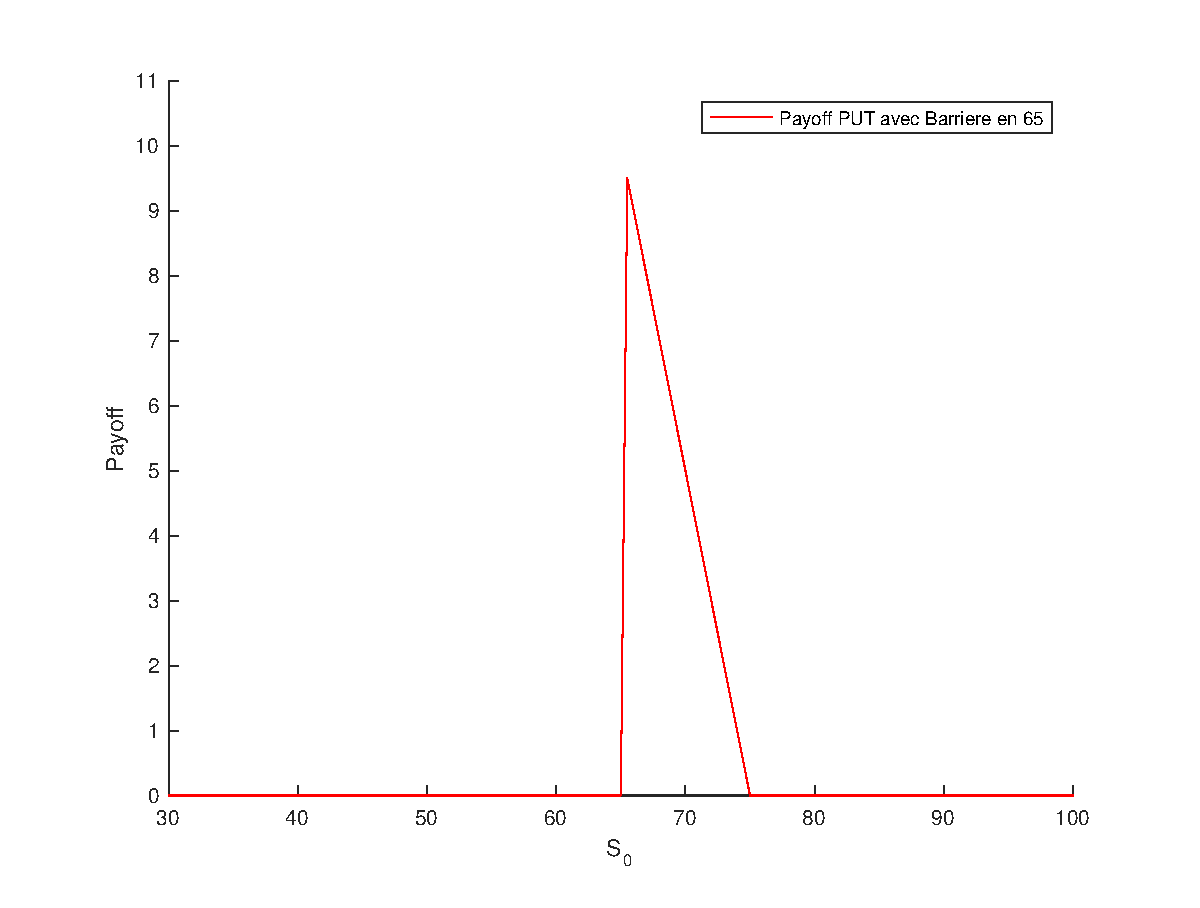
\includegraphics[scale=0.5]{./img/PUT_BAR_PAYOFF.eps}
\caption{Payoff d'une option barrière sur un PUT européen  en fonction du cours du sous-jacent}
\label{fig:put_bar_payoff}
\end{figure}

\begin{figure}[H]
\centering
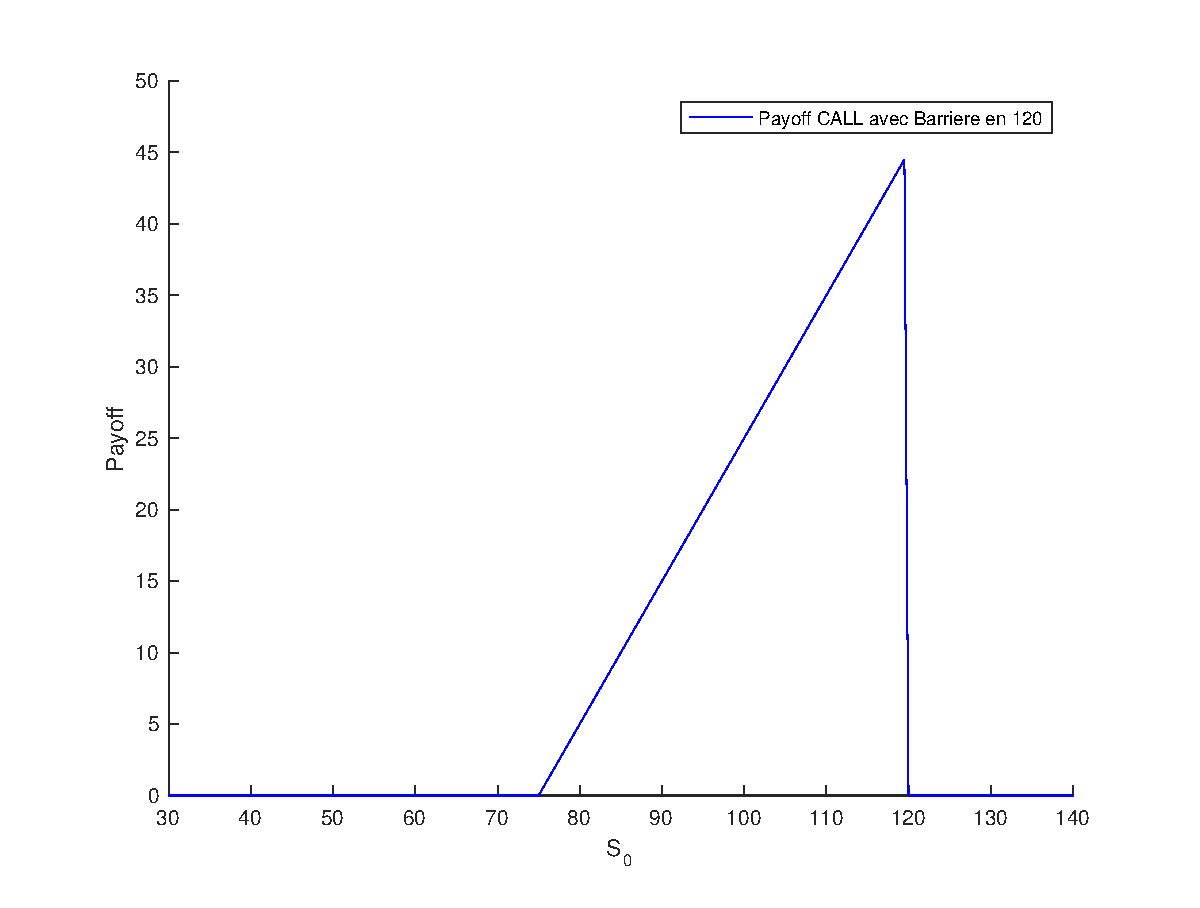
\includegraphics[scale=0.5]{./img/CALL_BAR_PAYOFF.eps}
\caption{Payoff d'une option barrière sur un CALL européen  en fonction du cours du sous-jacent}
\label{fig:call_bar_payoff}
\end{figure}

\subsection{Méthode de Monte-Carlo} % (fold)

\label{sub:methode_de_monte_carlo}

On analyse le prix de l'option en réalisant l'approximation de Monte-Carlo. La fonction pour le réaliser est Listing~\ref{listing:7}, le fichier dans lequel on la implémentée est \textsc{option$\_$barriere.py}. Les Figure~\ref{fig:call_put__bar_mc_tir}, Figure~\ref{fig:call_put_bar_mc} présentent les résultats obtenus.

\begin{figure}[H]
\centering
\includegraphics[scale=0.6]{./img/CALL_PUT_BAR_MC_TIR.eps}
\caption{Variation d'une option européenne avec option barrière approché par la méthode de Monte-Carlo en fonction du nombre de tirages}
\label{fig:call_put__bar_mc_tir}
\end{figure}

\begin{figure}[H]
\centering
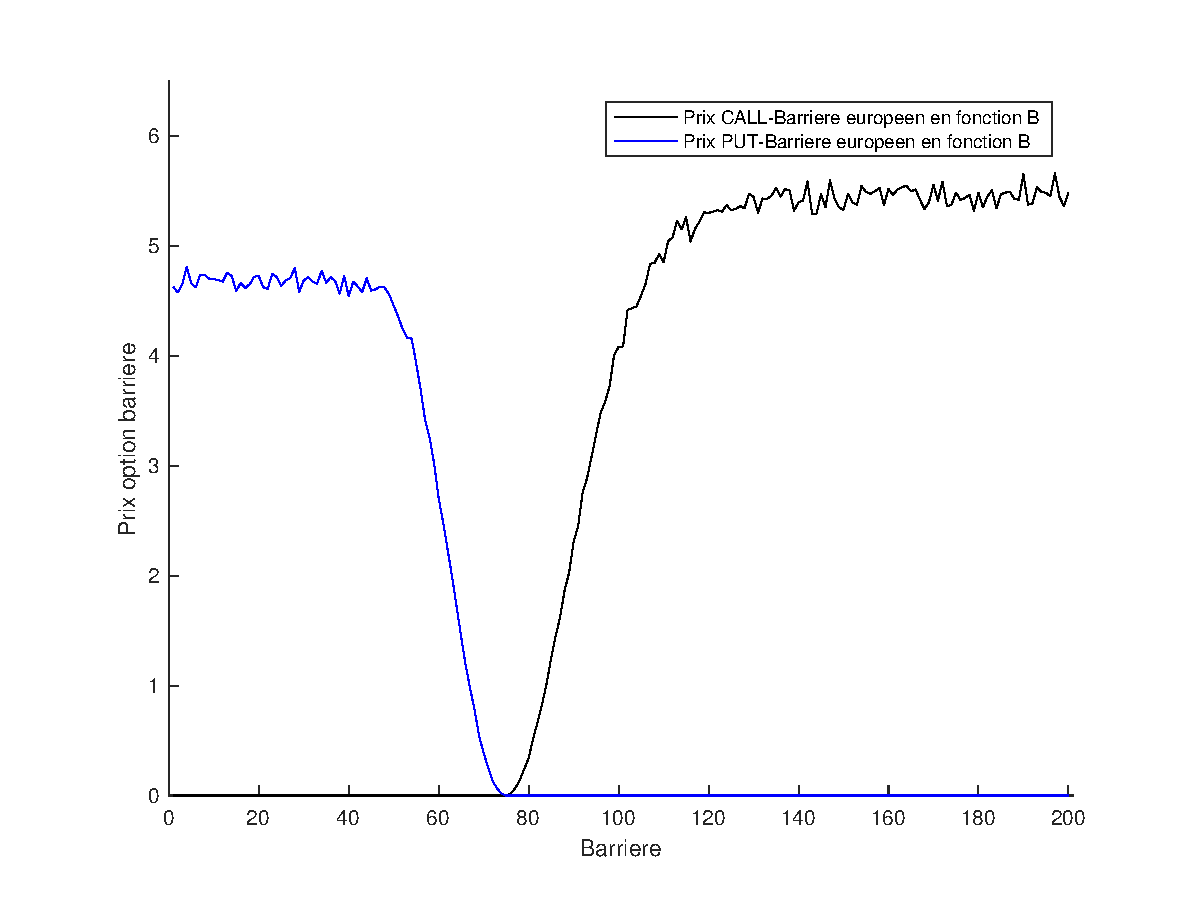
\includegraphics[scale=0.6]{./img/CALL_PUT_BAR.eps}
\caption{Variation d'une option européenne avec option barrière approché par la méthode de Monte-Carlo en fonction du niveau de la barrière}
\label{fig:call_put_bar_mc}
\end{figure}
% subsection methode_de_monte_carlo (end)

On peut voir que le prix du CALL augmente avec le niveau de la barriere et pour un barriere très grande, le prix est celui du modèle Black and Scholes. Pour le Put c'est exactement le contraire. Ce qui est logique, en effet si on pose la barrière très en dessous du prix \emph{At the Money} dans le cas d'un CALL, il est presque impossible que l'on ai un gain. Un raisonement similaire peut se faire pour le PUT.

On voit que le prix du PUT est inferieur au prix du CALL, car l'espérance de gain est inférieure.

\newpage

\subsection{Modèle Binomial} % (fold)
\label{sub:modele_binomial}

On analyse le prix de l'option dans le cadre du modèle binomial. La fonction pour le réaliser est Listing~\ref{listing:8}, le fichier dans lequel on la implémentée est \textsc{option$\_$barriere.py}. Les Figure~\ref{fig:call_put_bar_mb_prof}, Figure~\ref{fig:call_put_bar_mb} présentent les résultats obtenus.


Il est intéressant d'analyser comme sur la Figure~\ref{fig:call_put_bar_mb_prof} il y a plus de variations du PUT. La raison apparait sur la Figure~\ref{fig:call_put_bar_mb}, en effet on peut observer que pour un niveau de la barrière à 65, le delta du PUT est plus élevé que celui du CALL pour un niveau égal à 120.

\begin{figure}[H]
\centering
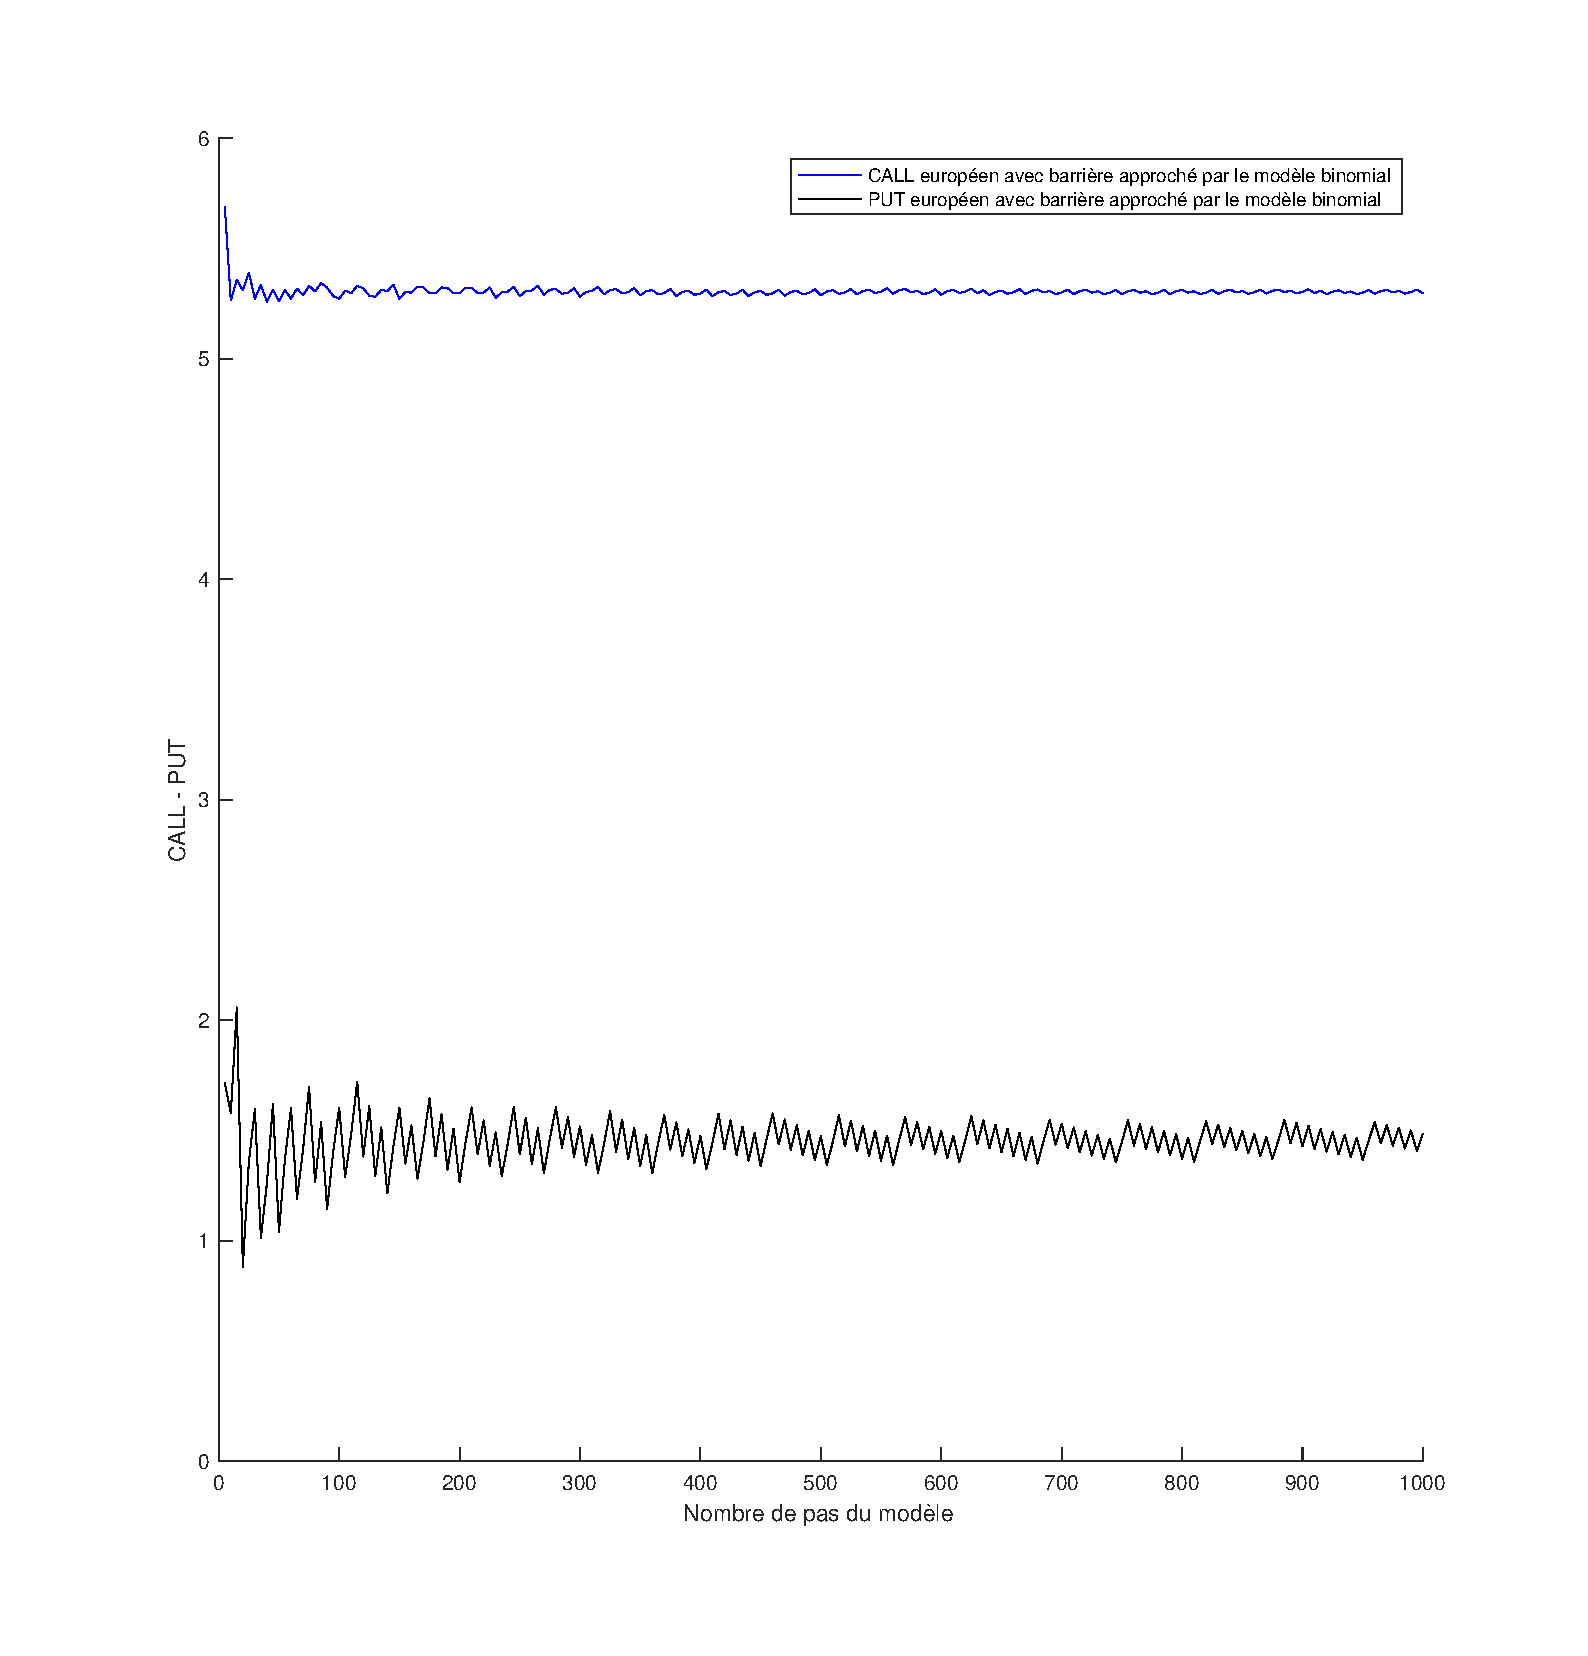
\includegraphics[scale=0.5]{./img/CALL_PUT_BAR_MB_PROFONDEUR.eps}
\caption{Variation d'une option européenne avec option barrière approché par le modèle binomial en fonction du pas}
\label{fig:call_put_bar_mb_prof}
\end{figure}

\begin{figure}[H]
\centering
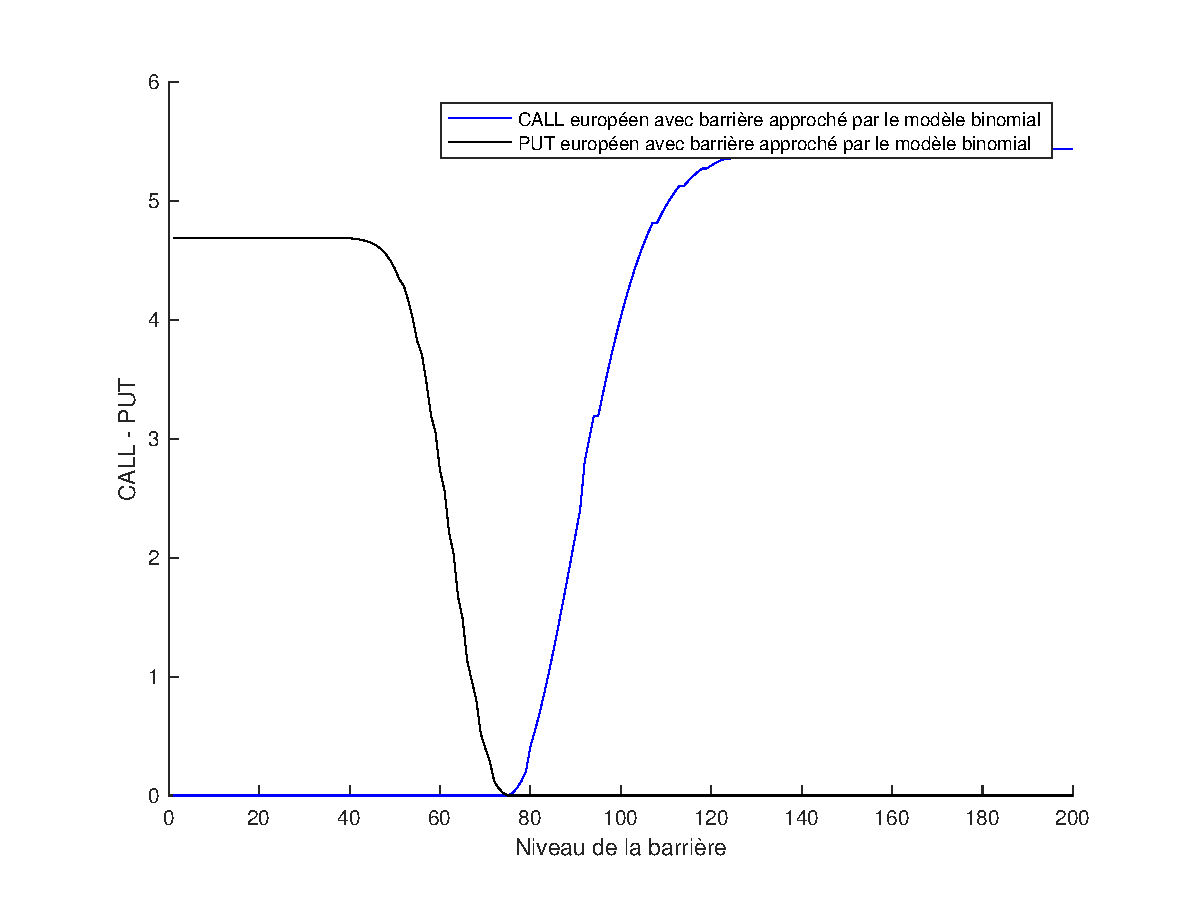
\includegraphics[scale=0.6]{./img/CALL_PUT_MB_BAR.eps}
\caption{Variation d'une option européenne avec option barrière approché par le modèle binomial en fonction du niveau de la barrière}
\label{fig:call_put_bar_mb}
\end{figure}

Les remarques sur les variations en fonction du PUT son les mêmes que dans le cadre Monte-Carlo. De plus on observe un lissage plus important, en effet la méthode de Monte-Carlo nécessite plus de tirages pour obtenir un résultat équivalent au modèle binomial. Cependant le grand avantage de la méthode de Monte-Carlo est que l'on n'a pas besoin de connaitre le modèle pour obtenir des résultats.

% subsection modele_binomial (end)

% section option_barriere (end)
\newpage

\section{Codes} % (fold)
\label{sec:codes}


\begin{listing}[H]
\inputminted[linenos,frame=leftline,breaklines=true,fontsize=\footnotesize]{matlab}{./codes/black_scholes.m}
\caption{Calcul du CALL et du PUT via la méthode de Black and Scholes. Matlab.}
\label{listing:10}
\end{listing}

\begin{listing}[H]
\inputminted[linenos,frame=leftline,breaklines=true,fontsize=\footnotesize]{matlab}{./codes/grecques.m}
\caption{Calcul des grecques du CALL dans le modèle de Black et Scholes}
\label{listing:11}
\end{listing}

\begin{listing}[H]
\inputminted[linenos,frame=leftline, breaklines=true,fontsize=\footnotesize]{python}{./codes/valeurs.py}
\caption{Fonction de calcul des valeurs nécessaires au modèle binomial}
\label{listing:1}
\end{listing}


\begin{listing}[H]
\inputminted[linenos,frame=leftline,breaklines=true,fontsize=\footnotesize]{python}{./codes/simul_arbre.py}
\caption{Simulation du payoff aleatoire dans le modèle binomial}
\label{listing:2}
\end{listing}


\begin{listing}[H]
\inputminted[linenos,frame=leftline,breaklines=true,fontsize=\footnotesize]{python}{./codes/modelebinomial.py}
\caption{Algorithme de calcul du prix d'une option via le modèle binomial}
\label{listing:3}
\end{listing}

\begin{listing}[H]
\inputminted[linenos,frame=leftline,breaklines=true,fontsize=\footnotesize]{python}{./codes/frontiere.py}
\caption{Calcul de la frontiere d'exercice d'une option americaine (temps,$S_t$)}
\label{listing:12}
\end{listing}


\begin{listing}[H]
\inputminted[linenos,frame=leftline,breaklines=true,fontsize=\footnotesize]{python}{./codes/delta_binomial_diff.py}
\caption{Algorithme de calcul du delta d'une option via le modèle binomial}
\label{listing:4}
\end{listing}

\begin{listing}[H]
\inputminted[linenos,frame=leftline,breaklines=true,fontsize=\footnotesize]{python}{./codes/montecarlo_bon.py}
\caption{Algorithme de calcul du prix d'une option europénne via la simulation de Monte-Carlo}
\label{listing:9}
\end{listing}

\begin{listing}[H]
\inputminted[linenos,frame=leftline,breaklines=true,fontsize=\footnotesize]{python}{./codes/delta_montecarlo.py}
\caption{Algorithme de calcul du delta d'une option europénne via la simulation de Monte-Carlo}
\label{listing:6}
\end{listing}

\begin{listing}[H]
\inputminted[linenos,frame=leftline,breaklines=true,fontsize=\footnotesize]{python}{./codes/option_bar_mc.py}
\caption{Algorithme de calcul du prix d'une option barrière via la simulation de Monte-Carlo}
\label{listing:7}
\end{listing}

\begin{listing}[H]
\inputminted[linenos,frame=leftline,breaklines=true,fontsize=\footnotesize]{python}{./codes/option_bar_mb.py}
\caption{Algorithme de calcul du prix d'une option barrière via le modèle binomial}
\label{listing:8}
\end{listing}

% section codes (end)

\end{document}